\documentclass[a4paper,11pt]{book}
%\usepackage{ml2k}
%\usepackage{epsf}
%\usepackage{mlapa}
%\usepackage[pdftex, colorlinks=true, citecolor=black, citebordercolor={.99 .99 .99}, linkbordercolor={.99 .99 .99}, pdfborder={0 0 1 [3]}]{hyperref}
\usepackage[pdftex, citebordercolor={.99 .99 .99}, linkbordercolor={.99 .99 .99}, pdfborder={0 0 1 [3]}]{hyperref}

\usepackage[fixlanguage]{babelbib}
\selectbiblanguage{spanish}

\usepackage[spanish, activeacute]{babel}
\selectlanguage{spanish}

% PRINT version
%\setlength{\oddsidemargin}{-20pt}
%\setlength{\evensidemargin}{-20pt}
%\setlength{\marginparwidth}{57pt}
%\setlength{\footskip}{30pt}
%\addtolength{\textwidth}{146pt}

% BOOK version
\setlength{\oddsidemargin}{53pt}
\setlength{\evensidemargin}{53pt}
\setlength{\marginparwidth}{57pt}
\setlength{\footskip}{30pt}


\usepackage[sort]{natbib}
\usepackage{psfrag}
\usepackage{fancyhdr}
\usepackage{appendix}
\usepackage{layout} 
\usepackage{graphicx} % para incluir graficos
\usepackage{amsmath} 
\usepackage{amsthm} % para escribir teoremas lindos
\usepackage{amsfonts} % para tener el simbolo de los numeros reales
\usepackage{color}  % colores de las fuentes

\usepackage{listings} % algoritmos
\lstdefinelanguage{chanfle}{	    
 	 morecomment=[l]{//},
 	 morecomment=[s]{/*}{*/},
   literate={:=}{{$\gets$}}1
   					{<-}{{$\gets$}}1
            {/not}{{$\neg$}}1
            {/and}{{$\land$}}2
            {/andThen}{{$\land_L$}}2
            {/or}{{$\lor$}}2
            {/orThen}{{$\lor_L$}}2
            {/imp}{{$\Rightarrow$}}2
            {/impThen}{{$\Rightarrow_L$}}2
            {/conjVacio}{$\emptyset$}1
            {/alpha}{$\alpha$}1
            {/alfa}{$\alpha$}1
            {->}{$\rightarrow$}2
            {NULL}{\sc{null}}4,
   keywords={if,for,then,else,while,fi,wend,true,false,var,case,of,esac,in,out,inout},
}

\lstnewenvironment{algoritmo}{}{}

\lstset{
	language=chanfle,
	basicstyle=\small,
	flexiblecolumns=false,
	basewidth={0.5em,0.45em},
	keywordstyle=\bfseries,
	tabsize=4
}

% Redefine plain page style
\fancypagestyle{plain}{
\fancyhf{}
\renewcommand{\headrulewidth}{0pt}
\fancyfoot[LE,RO]{\thepage}
}

% Code for creating empty pages
% No headers on empty pages before new chapter
\makeatletter
\def\cleardoublepage{\clearpage\if@twoside \ifodd\c@page\else
    \hbox{}
    \thispagestyle{plain}
    \newpage
    \if@twocolumn\hbox{}\newpage\fi\fi\fi}
\makeatother \clearpage{\pagestyle{plain}\cleardoublepage}

% Define pagestyle
\pagestyle{fancy}
\fancyhf{}
\renewcommand{\chaptermark}[1]{\markboth{ \emph{#1}}{}}
\fancyhead[LO]{}
\fancyhead[RE]{\leftmark}
\fancyfoot[LE,RO]{\thepage}

% Detalle de la TOC
\setcounter{tocdepth}{1}


\theoremstyle{definition} \newtheorem{axiom}{Axioma}
\theoremstyle{theorem} \newtheorem{teorema}{Teorema}

\begin{document}
\bibliographystyle{plainnat}
\bibpunct{(}{)}{,}{a}{,}{,}

\makeatother
\newcommand{\Nat}{\mathbb{N}}
% intervalo melodico
\newcommand{\IM}[1]{\underline{#1}}
\newcommand{\cita}{\textcolor{red}{cita}}
\newcommand{\alert}[1]{\footnote{\textcolor{red}{#1}}}
\newcommand{\red}[1]{\textcolor{red}{#1}}

%\newcommand{\alert}[1]{\textcolor{red}{#1}}
\newcommand{\mycomment}[1]{\textcolor{blue}{#1}\newline}
%\renewcommand{\comment}[1]{\ }
\theoremstyle{definition} \newtheorem{definition}{Definici'on}


\newcommand{\defaultAlignment}{center}
\newcommand{\defaultWidth}{12.5cm}
\newcommand{\defaultPosition}{h}
\newenvironment{imagen}{
\let\File\empty
\let\Desc\empty
\let\LabelName\empty
\let\Width\textwidth
\let\Alignment\defaultAlignment
\let\Position\defaultPosition
}{
    \begin{figure}[\Position]
    \begin{\Alignment}
    \includegraphics[width=\Width]{\File}
    \caption{\Desc}
    \label{\LabelName}
    \end{\Alignment}
    \end{figure}

}

\newcommand{\position}[1]{\def\Position{#1}}
\newcommand{\file}[1]{\def\File{#1}}
\newcommand{\desc}[1]{\def\Desc{#1}}
\newcommand{\labelname}[1]{\def\LabelName{#1}}
\newcommand{\width}[1]{\def\Width{#1}}
\newcommand{\alignment}[1]{\def\Alignment{#1}}


%\begin{abstract}
%asd
%\end{abstract}

\frontmatter

%\title{Hacia una validaci\'on generativa de teor\'ias cognitivas musicales}
\author{Pablo Hern\'an Rodr\'iguez Zivic}
\date{}
\maketitle

\thispagestyle{empty}

\begin {center}


\includegraphics[scale=.3]{uba2.jpg}

\medskip
UNIVERSIDAD DE BUENOS AIRES

Facultad de Ciencias Exactas y Naturales


\vspace{3cm}


\textbf{\Large Hacia una validaci\'on generativa de teor\'ias cognitivas musicales}

\vspace{2cm}



\vspace{2cm}

\textbf{Pablo Hern\'an Rodr\'iguez Zivic}

\end {center}


\vspace{1.5cm}

\noindent Director de tesis: Carlos Diuk

\noindent Co-director: Favio Shifres 


\vspace{1cm}

\vspace{1cm}

\noindent Buenos Aires, 2009



%\section*{Agradecimientos}
La lista de agradecimientos realmente es s'uper larga. Creo que en mayor o menor medida, todos los que estuvieron cerca mio este 'ultimo a~no de alguna forma
aportaron a que ahora s'olo me falte escribir los agradecimientos. \newline

Si bien es verdad que todos los que estuvieron cerca mio en cierta forma me ayudaron, hay varias personas que vale mencionar. \newline

Los primeros son mis queridos viejos: Mam'a y Pap'a, m'as conocidos como Silvia Zivic y Carlos Rodriguez. Estoy muy agradecido de todo el vuelo que me ayudaron a tomar
desde que recuerdo: estoy convencido de que gran parte de todo esto fue gracias a que mi papi me ense~n'o la Ley de Ohm cuando ten'ia unos 7 a~nos, 
y mami me ense~n'o a tocar el piano cuando ten'ia unos 4 a~nitos.\newline

Tambi'en quiero agradecer a los pibe'$\ $ de la facu, no podr'ia haber aprendido todo lo que aprend'i si no fuera por ellos: trabajamos y nos divertimos juajuaja. 
Posta, gracias a PabloB, Lata, el Sabi, Jota, Luigi, la Topa, Piter, Droopy, Toto, Guidh'in, el Roque~no y Eze.\newline

No me olvido de ustedes, no se pongan celosos, tal vez ahora no nos vemos tanto, pero son como mi familia: Noe, Moni, Henry, Armandito, Melu, Ceci, Nati, Adri y 
Gianni. \newline

Jime, te quiero mencionar aparte. Me ayudaste un mont'on en un momento s'uper duro, y gracias a eso pude poner distancia y mirar friamente para darle
un punto final a este trabajo. !`Gracias por estar siempre! \newline

No hay que quitarle m'erito a todos los que padecieron las primeras composiciones de la compositora: si ahora no es placentero escucharla, imaginate antes. 
Esta gente es basicamente la que comparte mi d'ia a d'ia: El Mono, Diego, Santi H., Vic, Manu, Bru, Edu, Cono, Tom, Luiso, Coni, Fer (Zuzuzuzunino!), 
Santi Coffey y Santi Siri.\newline

Mis queridos directores que se bancan mis rayes, mis explociones de mails, mis terquedades, y todas esas cualidades tan lindas con las que tienen que lidiar: 
Gracias Favio!, Gracias Greg!\newline

Adem'as hay que bancarse leer estas 85 p'aginas, !`Gracias a Agust'in y a Pablo por dedicarme ese tiempo!\newline

\begin{center}
\LARGE{!`Gracias!}
\end{center}

%\section{Abstract}

%\include{msc_titlepage}
%\include{msc_preface}
%\include{msc_summary}

% Remove parskip for toc
\setlength{\parskip}{0ex plus 0.5ex minus 0.2ex}
\tableofcontents

\mainmatter
% Adjustments headers
\fancyhead[LO]{\leftmark}
\fancyhead[RE]{\emph{Cap\'itulo \thechapter}}


\chapter{Introducci\'on}
\section{Introducci\'on y objetivos}
Hacia fines del siglo XIX y principios del siglo XX (\alert{revisar}), con el prop'osito de estudiar la estructura interna de una pieza musical, 
Heinrich Schenker elabor'o un m'etodo de an'alisis musical conocido como \texttt{an'alisis schenkeriano}.
Esta estructura es descripta por el autor en t'erminos de \texttt{reducciones}. Una reducci'on permite especificar que una cierta nota dentro de un grupo es la fundamental, 
y que todo el resto es una \texttt{elaboraci'on} de esta. Dado que esta relaci'on de reducci'on/elaboraci'on se puede aplicar recursivamente, naturalmente emerge una relaci'on 
jer'arquica entre las notas de una pieza musical.  En esta jerarqu'ia, el nivel m'as bajo es lo que se encuentra escrito en la partitura, y a medida que se sube de nivel se 
encuentra la misma pieza musical, pero carente de elaboraciones. A continuaci'on se excibe un ejemplo de dicho an'alisis:


\begin{figure}[h]
\begin{center}
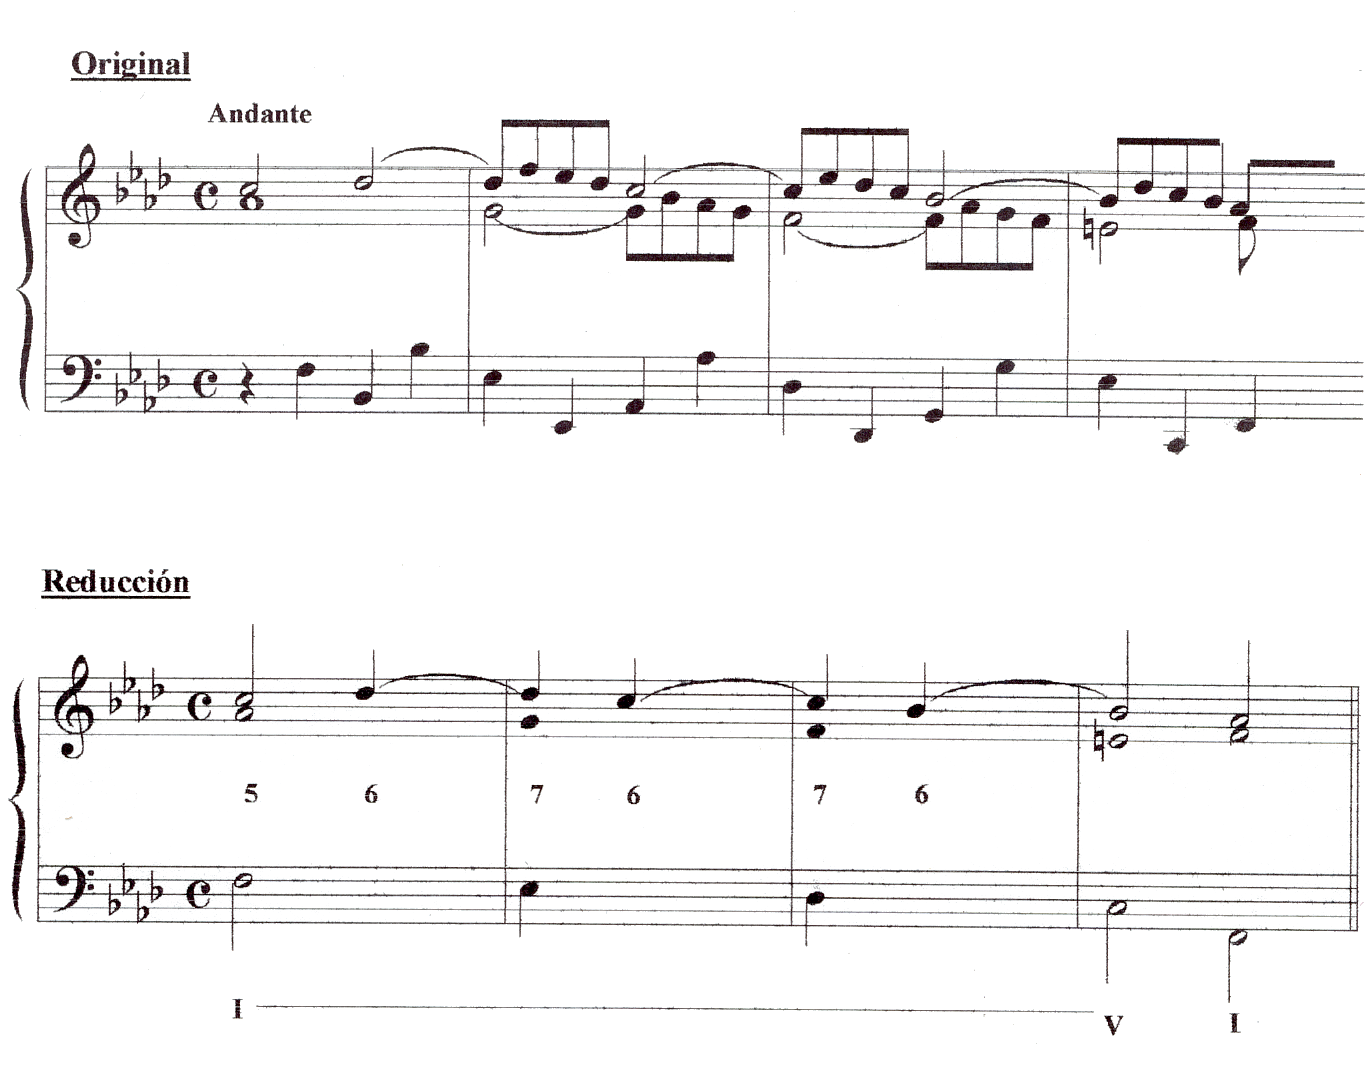
\includegraphics[width=12cm]{images/schenkerian_example.png}
\newline \alert{poner una imagen mas copada}
\end{center}
\end{figure}

En esta figura, los sucesivos pentagramas muestran relaciones de reducci'on, as'i simplificando el tema con el objeto de llevarlo a una representaci'on mas concreta.

El parecido de este tipo de relaciones con las relaci'ones utilizadas por Noam Chomsky para analizar el lenguaje natural es notable. 
Si bien en la teor'ia de Chomsky las relaciones son relaciones del tipo ``es un'', y en la teor'ia de Schenker son del tipo ``es una elaboraci'on de'', 
estas se enmarcan matem'aticamente en el mismo lugar.  

En 1983, el m'usico Fred Lerdahl y el ling\"uista Ray Jackendoff publicaron el libro 
\texttt{A Generative Theory of Tonal Music}(GTTM) donde proponen una gram'atica para analizar la m'usica t'erminos parecidos a los de Schenker. 
Lo hace interesante a este trabajo es el fundamento que se le da a la elecci'on de las reglas de la gram'atica, puesto que analizan la teor'ia 
schenkeriana en t'erminos cognitivos.  

El objetivo del trabajo de Lerdahl y Jackendoff es principalmente tener un modelo que sea capaz de describir el proceso mediante el cual se estructura la percepci'on de la m'usica. 
Este modelo consiste en una serie de reglas de preferencia. Cada regla tiene asociado un predicado booleano $P$ y un valor de preferencia $v$, 
de modo que si el predicado booleano es verdadero, entonces aportan $v$ unidades a la preferencia de una cierta acci'on interpretativa. Para ejemplificar, a continuaci'on se cita
una regla de preferencia de los autores. Esta regla es una de las reglas asociadas a lo que los autores llaman agrupamiento, que b'asicamente consiste en agrupar notas que tienen
significancia de frase\footnote{M'as adelante se explicar'a esto con mayor detalle}.
\newline

\begin{center}
\texttt{GPR 1} Evite fuertemente grupos que contengan solamente un evento.
\end{center}

En este caso, el predicado booleano es aquel que es verdadero solamente con grupos de cardinalidad uno, y el valor de preferencia es fuertemente negativo a la acci'on interpretativa
de decidir que el grupo en cuesti'on debe contener 'unicamente al evento que contiene. Como esta, los autores exiben un gran conjunto de reglas que luego validan experimentalmente. 

Si bien un modelo de este tipo es generativo en el sentido de que podr'ia ser utilizado por una computadora tanto para analizar una pieza musical como para 
\texttt{generar} una nueva, es importante notar que este no es su objetivo. 
Puede verse claramente como la regla \emph{GPR 1} si bien es suficientemente rigurosa como para luego poder corroborarla emp'iricamente, no lo es como para construir un 
programa que haga un an'alisis utilizando esta regla: es necesario determinar el valor de preferencia y aprender las relaci'ones entre los distintos valores de preferencia para luego 
tomar una desici'on.  

De esta forma se discrimina entre \texttt{modelos generativos}, que son aquellos que eventualmente podr'ian utilizarse para generar aquello que explican, y 
\texttt{modelos de 'indole generativo} que fueron hechos con el objeto de generar aquello que explican.  El hecho de que sea necesario definir expl'icitamente los valores de preferencias
sumado a que este modelo no es de 'indole generativo plantea el interrogante de si realmente este enfoque es el adecuado para para modelar la cognici'on musical con aprendizaje 
autom'atico. 

De este modo, el objetivo de este trabajo es utilizar el conocimiento generado por trabajos como el de Lerdahl y Jackendoff como medio para establecer propiedades que un modelo de 
'indole generarivo deber'ia cumplir. Teniendo estas propiedades, luego es posible construir un modelo desvinculado con la idea de gram'atica, pero que respete 
ciertos criterios fundamentales. Si se logra conseguir un modelo de estas caracter'isticas se podr'an validar emp'iricamente los criterios en base a los que el modelo fue construido 
(y por lo tanto las teor'ias cognitivas motivaron los criterios) a trav'es de analizar las piezas musicales generadas por el modelo.

Para poder avanzar en pos del objetivo recien planteado, es necesario primero sentar un vocabulario para luego poder contextualizarlo. De esta forma, las siguientes dos
secci'ones hablaran sobre background. Luego se har'a un breve resumen sobre el estado del arte en este tema, para luego abordar el trabajo en concreto de esta tesis.


\section{Aportes de este trabajo}
Se considera como aporte principal de este trabajo la metodolog'ia de validaci'on propuesta: 

Contando con modelos generativos aislados para distintos atributos musicales, es posible validar los fundamentos de cada modelo
realizando una serie de composiciones en donde se ve afectando el funcionamiento del modelo correspondiente.

Para poder alcanzar este objetivo, fue necesario construir modelos ge\-nerativos con base en teor'ias psicol'ogicas para los distintos atributos que 
caracterizan a una melod'ia. 

De este modo, la contribuci'on de este trabajo se sintetiza en la siguiente lista de modelos (muchos de los t'erminos relacionados con teor'ia musical se definir'an
m'as adelante):

\begin{itemize}
 \item Modelo para la r\'itmica: Basado en 3 propiedades perceptuales del acento m'etrico, fue posible construir un modelo sencillo para la r'itmica
 que cumpla con la propiedad de que la r'itmica generada har'a que un oyente infiera la misma estructura m'etrica que la que el 
 oyente inferir'ia en la obra original.

 \item Modelo para los contornos mel'odicos: Basado en la teor'ia de Implicaci'on-Realizaci'on de \cite{Narmour90}, se propone un modelo simple que permite cuantificar 
 el grado de implicaci'on que genera un intervalo mel'odico sobre el siguiente.

 \item Modelo para contextos arm'onicos: Basado en los trabajos de \cite{Krumhansl90} y \cite{Lerdahl2001} se propone un modelo basado en un marco bayesiano
 para cuantificar la estabilidad de una nota en funci'on de la tonalidad inferida del tema y el acorde que gobierna la sonoridad del momento.

 \item Modelo para frases mel'odicas: Utilizando los modelos anteriores, y basado en algunas definici'ones de en qu'e consiste una 
 frase musical, se construye un modelo que organize la melod'ia en t'erminos de unidades discursivas.

 \item Modelos para generar relaciones mot'ivicas: Se propone utilizar el modelo de los Restaurantes Chinos \citep{Teh2007} para generar repetici'on 
 de partes, de forma tal que la cantidad de repeticiones de una parte no sea excesiva ni nula.

\end{itemize}


A modo de resumen, en la figura \ref{fig:arquitectura} se exhibe la arquitectura de los modelos utilizados y en qu'e cap'itulo se aborda cada uno.

\begin{imagen}
    \file{images/arq.png}
    \labelname{fig:arquitectura}
    \desc{Descripci'on gr'afica de la arquitectura utilizada}
    \width{10.5cm}
    \position{!h}
\end{imagen}

\begin{itemize}
 \item Pitch Profile: Construye el pitch profile definido en la secci'on \ref{sec:pitch_profile}.
 \item Chord Detection: Aplica una heur'istica para detecci'on de acordes.
 \item Contour Patterns: Calcula el modelo definido en la secci'on \ref{sec:contour_model}.
 \item Notes Distribution: A partir del Pitch Profile y del acorde actual construye la distribuci'on de notas que aplica al contexto actual seg'un lo definido en la secci'on \ref{sec:harmonic_context_model}.
 \item Phrase Repetition: Utilizando el Restaurant Chino correspondiente al acorde actual, se elije un identificador para la parte actual como 
 se defini'o en la secci'on \ref{sec:crp_model}.
 \item Phrase Rhythm: Utilizando la duraci'on determinada por el acorde actual y el identificador determinado por la etapa de Phrase Repetition se 
 genera una frase r'itmica como se defini'o en la secci'on \ref{sec:rythm_model}.
 \item Pitch Phrase: Utilizando la r'itmica generada por la etapa de Phrase Rhythm, se asignan notas utilizando como contexto arm'onico el determinado 
 por Notes Distribution y utilizando como restricci'ones para el contorno mel'odico las determinadas por Contour Patterns utilizando 
 el algoritmo definido en la secci'on \ref{sec:phrase_model}.
\end{itemize}


\section{Estado del arte}
\label{sec:state_art}
A continuaci'on se har'a un breve resumen sobre los distintos enfoques y objetivos relacionados con el an'alisis musical mediante
t'ecnicas computacionales. Las aplicaciones de este tipo de trabajos son bastante variadas, tales como herramientas para 
composici'on musical asistida, acompa~namiento autom'atico, indexaci'on de m'usica, sistemas de recomendaci'on musical e 
investigaci'on en psicolog'ia de la m'usica, donde se sit'ua este trabajo.

De acuerdo al enfoque que se tome, puede variar la representaci'on musical utilizada entre la se~nal sonora cruda, 
y una partitura\footnote{o midi, que es equivalente a niveles pr'acticos }.
En este trabajo se asumir'a una representaci'on simb'olica de la m'usica para poder desarrollar en profundidad las teor'ias cognitivas de las 
que luego se hablar'a. A continuaci'on se nombran algunos trabajos que se enmarcan de la misma forma en t'erminos de la representaci'on musical.

\cite{PaieThesis} propone un modelo generativo para l'ineas mel'odicas, 
patrones r'itmicos y armonizaci'ones, basado en algunos de los principios que se utilizar'an en este trabajo. 
Sin embargo, no es el objetivo del autor poner a prueba teor'ias cognitivas de la m'usica; sino desarrollar un modelo generativo,
y por lo tanto predictivo, basado en una representaci'on simb'olica de la m'usica de forma tal que se pueda utilizar el conocimiento generado por estos
modelos para mejorar la calidad de algoritmos que trabajan con se~nales sonoras. Este trabajo aborda el problema de la estabilidad tonal a partir
de entrenar una cadena de Markov que tiene estados ocultos que representan los acordes, aspecto que puede ser abordado utilizando las teor'ias 
de \cite{Krumhansl90} y \cite{Lerdahl2001}. De la misma manera, el modelo de la r'itmica utiliza una definici'on incorrecta de acento m'etrico, asumiendo
que tiene caracter'isticas globales. Si bien estos modelos podr'ian funcionar en el marco en el que el autor los plantea, en este marco no son de utilidad.

\cite{Shih-Chuan} proponen un software que mediante la utilizaci'on de t'ecnicas de data mining componga m'usica. Estas t'ecnicas son aplicadas
para descubrir patrones en la composici'on musical en su estructura r'itmica y mel'odica.
Si bien estos modelos no son de inter'es para este trabajo por no basarse directamente en fundamentos cognitivos, 
la arquitectura que presentan \cite{Shih-Chuan} sirvi'o como punto de partida para construir la presentada en este trabajo. 

Otro software existente dise~nado para componer m'usica es el Melisma Music Generator
\footnote{Disponible en http://www.link.cs.cmu.edu/melody-generator/} basado en \cite{Temperley2004}. 
Este software se encuentra disponible para escuchar online sus composiciones, presentando una interfaz web donde es posible ingresarle distintos
valores a sus par'ametros y escuchar como estos impactan en la composici'on final. 
El mayor problema 
que tiene es que no se puede entrenar directamente su modelo con una partitura, y por m'as que se intentara realizar esto construyendo un software 
que estime valores posibles para sus par'ametros, no habr'ia forma de determinarle ciertos par'ametros que son utilizados en este trabajo, 
como la sucesi'on de contextos arm'onicos.


%David Cope, en trabaja con un software, que mediante reglas, sea capaz de reproducir el estilo de una pieza musical dada. Si bien 
%la construcci'on ha sido exitosa en algunos casos, generando composiciones que realmente respetan el estilo de la pieza original, gran
%parte de las reglas utilizadas no tienen sustento cognitivo.
%

\cite{Cambouropoulos98} propone una teor'ia general para el an'alisis musical. 
Su trabajo consiste en una teor'ia computacional que permitir'ia obtener una descripci'on de la estructura de una cierta obra musical. Si bien sus 
objetivos son distintos a los que se proponen aqu'i, no distan tanto: 
\begin{quote}
[\ldots]Teor'ias musicales permiten formular hip'otesis y modelos que pueden ser implementados
como programas para luego ser evaluados, y, de forma inversa, resultados de la aplicaci'on de
estos programas podr'ia forzar la re-examinaci'on y ajuste de las teor'ias iniciales. \footnote{[\ldots]Musical theories allow the formulation of hypotheses and models which can be implemented
as computer programs and then evaluated, and, conversely, results from the application of the
computer programs may force the re-examination and adjustment of the initial theories. [\ldots]
} [\ldots]

\end{quote} 
A lo largo de este trabajo no se utiliz'o esta teor'ia y se opt'o por teor'ias que han sido m'as ampliamente discutidas tanto en el marco de la musicolog'ia
como en el marco de la psicolog'ia de la m'usica.

%
%En \cite{Simon_mysong:automatic} mediante el an'alisis de caracter'isticas de la se~nal sonora correspondientes a una melod'ia 
%cantada, y mediante entrenar un Hidden Markov Model para la probabilidad de un acorde, dado que se observa una cierta nota cantada,
%se construy'o un sistema capaz de armonizar una melod'ia. Un sistema comercial que realiza esto mismo es Band-in-a-box,
%pero dado que no existen \red{revisar} publicaciones respecto a c'omo fue construido, no se puede hacer m'as que nombrarlo.
%
%Dentro de la rama de sistemas para indexar m'usica se situan trabajos como \cite{StructureAnalysis1}. En 
%\cite{StructureAnalysis1} se propone un m'etodo para analizar la estructura de una pieza musical a partir de su se~nal sonora. Esto lo logran extrayendo vectores 12-dimencionales
%de cada momento del tema, en donde cada componente del vector muestra la intencidad relativa de cada altura en ese momento, y a partir
%de estos vectores y una noci'on de distancia construyen matrices de similitud que permiten detectar los acordes que aparecen
%en el tema. Siguiendo con este 

El resto de la tesis se organiza de la siguiente forma: En el cap'itulo 2 se cubren superficialmente los conceptos b'asicos que el lector debe manejar para entender
este trabajo. Se alienta a los lectores no iniciados en alguna de las tem'aticas abordadas profundizar tales conceptos en la literatura referida. 
En el cap'itulo 3 se exhibe modelos que capturan dependencias a nivel local en la m'usica tonal. 
En el cap'itulo 4 se muestra modelos de 'indole jer'arquico y por 'ultimo en el cap'itulo 5 se reportan los experimentos realizados junto con 
las conclusiones del trabajo.

\chapter{Background}
\label{cap:background}
\section{Sobre notas, alturas, acordes y tonalidades}
\label{sec:musical_intro}
Esta secci'on tiene dos objetivos; por un lado, que el lector no familiarizado con teor'ia musical establezca
ciertos conceptos generales que son utilizados en el desarrollo de este trabajo y, por el otro, establecer un glosario
que se utilizar'a a lo largo de las diferentes secciones.

Principalmente, la m'usica tonal posee dos grandes dimensiones: el \texttt{tiempo} y la \texttt{altura}. 
La dimensi'on temporal responde a \emph{cu'ando} ocurre un evento, mientras que la altura expresa caracter'isticas sobre \emph{qu'e}
tipo de evento es. Por altura se refiere a la localizaci'on de un sonido en una escala tonal, dependiendo de la velocidad de las vibraciones de la fuente sonora; 
as'i las frecuencias r'apidas producen sonidos m'as agudos, y las lentas sonidos m'as graves \citep[p. 565]{kennedy1996oxford}.
Esta percepci'on si bien esta relacionada con caracter'isticas intr'insecas del sonido, como su intensidad, timbre y frecuencia, 
tambi'en hace referencia
al proceso cognitivo que ocurre por parte del oyente. De esta forma, si bien sonidos de $440\mbox{Hz}$ y $441\mbox{Hz}$ son distintos, 
perceptualmente se perciben de la misma forma, como la nota La.

En la m'usica occidental, existen criterios dentro de ambas dimensiones que ayudan a la organizaci'on de una pieza musical. 

Por 'ultimo, dado que a lo largo del presente trabajo se exhiben ejemplos, es necesario que el lector sepa comprender una partitura sencilla, 
de forma que se se explicar'a brevemente c'omo ciertos conceptos introducidos se anotan con el c'odigo convencional de escritura musical.

\subsection{Sobre la organizaci\'on temporal}
\label{sec:temporal_organization}

El primer concepto importante a tener en cuenta es que en la m'usica de caracter'isticas m'etricas el transcurrir del tiempo est'a \emph{discretizado}. Esto no quiere decir que a la hora de la producci'on musical lo sea, sino que, 
en la abstracci'on musical, existe una unidad de referencia temporal, a la que se denomina \emph{beat}. En torno a ella se organiza la estructura temporal, tocando
siempre notas que duren una fracci'on del mismo. De esta forma, para poder reproducir una partitura es necesario saber 
la duraci'on del \emph{beat} de referencia, denominado \emph{tempo}, luego el resto de las duraciones son una fracci'on de 'esta.


En \citet*{LerdahlJackendoff83} se hace una distinci'on entre dos estructuras que ocurren en simultaneidad en la m'usica tonal:
la estructura \emph{m'etrica} y la estructura del \emph{agrupamiento}\footnote{\emph{meter} y \emph{grouping} en ingl'es}. 
La estructura del agrupamiento hace referencia a la organizaci'on de una pieza musical en unidades que pueden ser motivos, frases, secciones, etc. 
Cada una de estas unidades, es denominada por los autores como \emph{grupo}. Asimismo, el oyente infiere una estructura \emph{regular} de beats. 
Algunos beats reciben una acentuaci'on mayor que otros, determinando lo que los autores definen como la estructura m'etrica. Dentro de esta estructura
existen distintos niveles, cada uno determinado por el tiempo transcurrido entre dos beats consecutivos. 
Se referir'a por contexto m'etrico de una pieza a la estructura m'etrica que se infiere a partir de esta.

Ambas estructuras son jer'arquicas, en el sentido de que existen sub-estructuras a distintos niveles, y que las sub-estructuras de niveles superiores 
incluyen por completo a las de nivel inferior
\footnote{Para una definici'on m'as formal de la jerarqu'ia referirse a \citet[cap. ~2]{LerdahlJackendoff83}}. De esta forma, una secci'on
de una pieza musical estar'a formada por una sucesi'on de frases. Cada frase pertenecer'a s'olo a una secci'on aunque distintas repeticiones de la misma
frase pertenecer'an potencialmente a distintas secciones. Obs'ervese que con esta definici'on, los niveles altos en la jerarqu'ia corresponen a 
porciones m'as largas en el tema. 

Respecto a la estructura m'etrica, la noci'on de jerarqu'ia es menos evidente. En la definici'on original, los autores utilizan una representaci'on geom'etrica
por el simple hecho que una \emph{m'etrica} tiene sentido cuando hay algo que medir. De esta forma, utilizando esta met'afora geom'etrica, los autores representan 
a los beats como puntos sin duraci'on. Luego definen el concepto de \emph{time-span} como el tiempo entre dos beats sucesivos. 
La relaci'on entre un beat fuerte, y su posici'on en la jerarq'ia m'etrica es simplemente la siguiente: si un beat se escucha m'as fuerte que el siguiente, eso implica
que el primero est'a en un nivel mayor que el segundo.

%\red{este parrafo no est'a bien, lo dejo para acordarme de reescribirlo}
%
%La organizaci'on jer'arquica de la m'usica no es una teor'ia solo postulada por Lerdahl y Jackendoff; Cooper y Meyer (\cite{CooperMeyer60}) plantean una teor'ia similar en
%estos t'erminos, Kramer (\cite{Kramer88}) si bien no habla directamente de una jerarqu'ia, propone que tienen un rol 
%estructurante\alert{tengo que leer m'as, as'i se mejor de lo que hablan estos dos muchachos}. 
%
%Un nivel de especial inter'es, es el denominado \emph{tactus}, que b'asicamente es el marcado por el director de orquesta al mover su batuta. 
%El tactus tambi'en es la distancia entre los beats que el oyente marca cuando mueve el pie y est'a relacionado con el baile. 
%
Es importante notar que esta estructura es ambigua, en el sentido de que muchas veces no existe un 'unico an'alisis de una pieza musical 
en una estructura m'etrica y de agrupamiento.

\begin{imagen}
    \file{images/metrical_structure2.png}
    \labelname{fig:metrical_structure}
    \desc{An'alisis de estructura m'etrica y de agrupamiento. Imagen tomada de \cite{LerdahlJackendoff83}. Los par'entesis inferiores representan
    a la estructura del agrupamiento. Los puntos representan la jerarqu'ia m'etrica: columnas con mayor cantidad de puntos representan un acento a un nivel 
    mayor.}
    \width{10cm}
\end{imagen}

En la figura \ref{fig:metrical_structure} se exhibe una partitura con un an'alisis m'etrico y de agrupamiento. 
No se pretende que el lector interprete esta figura por completo, sino mostrar c'omo estos dos an'alisis se aplican a una pieza musical. 
En esta figura se puede observar c'omo cada nivel de la estructura m'etrica determina un pulso regular, 
y los niveles inferiores subdividen a este tambi'en de forma regular. Tambi'en se puede ver la jerarqu'ia determinada por los dos an'alisis.


En cuanto a la duraci'on de las notas, dado que cada nota no puede tener una duraci'on arbitraria, y que esta duraci'on est'a relacionada con el tempo
a trav'es de una fracci'on, existen s'imbolos y nombres para diferentes duraci'ones. 
En la figura \ref{fig:durations} se muestran las figuras correspondientes a notas y silencios de distintas duraciones. De las figuras exhibidas, la relaci'on de duraci'ones
es siempre del doble con respecto a otra: la redonda dura el doble que una blanca, la blanca dura el doble que una negra, etc. 
Se denomina plica, a la barra vertical que surje 
de la cabeza de las notas, con excepci'on de la redonda. Es importante aclarar que cuando dos notas de duraci'on inferior o igual a una corchea se tocan seguidas, 
se unen las plicas (ver figura \ref{fig:example_measure}).

\begin{imagen}
    \file{images/note_values.jpg}
    \labelname{fig:durations}
    \desc{Figuras de ejemplo}
    \width{10cm}
\end{imagen}

Las partituras luego se organizan en una serie de unidades, cada una denominada \emph{comp'as}. Todos los compases tienen la misma duraci'on, y 'esta se especifica
en la partitura por una fracci'on al comienzo de la misma. Esta fracci'on no debe interpretar de forma usual, ya que posee una sem'antica sutilmente diferente.
En la especificaci'on del comp'as, el denominador determina en qu'e unidades se medir'a la longitud del comp'as, y el numerador determina cu'antas unidades 
durar'a. El valor de referencia para el denominador es el $4$ refiriendo a una negra, y m'ultiplos de este refieren a m'ultiplos de una negra. Por ejemplo
$8$ refiere a corcheas.  De esta forma, un comp'as de $\frac{3}{4}$ indica que la unidad de referencia es la negra, y que hay $3$ negras por comp'as.
La figura \ref{fig:time_signatures} muestra c'omo se especifican en una partitura los compases m'as comunes.

\begin{imagen}
    \file{images/Common_time_signatures.png}
    \labelname{fig:time_signatures}
    \desc{Compases comunes}
    \width{5cm}
\end{imagen}

Obs'ervese que a fines de notar la duraci'on del comp'as, no existe diferencia entre el comp'as de $\frac{3}{4}$ y el comp'as de $\frac{6}{8}$, su diferencia
radica en la acentuaci'on recibida por distintos eventos: En el comp'as de $\frac{3}{4}$, existen 3 eventos de negra, donde el primero se percibe como acentuado, 
y los dos siguientes se perciben como m'as d'ebiles, mientras que en el comp'as de $\frac{6}{8}$ hay 6 eventos, donde el primero es el m'as 
acentuado, luego sigue el cuarto, y por 'ultimo el resto de los beats. En la figura \ref{fig:acentos_compas} se exhiben los compases de $\frac{3}{4}$, $\frac{4}{4}$ 
y $\frac{6}{8}$ con sus respectivos an'alisis m'etricos. En esta figura, los niveles corresponden a distintos \emph{time-spans}, es decir, los beats 
que ocurren en el tercer nivel tienen un per'iodo mayor que los beats que ocurren en los niveles uno y dos. En el comp'as de $\frac{4}{4}$, 
el nivel inferior corresponde a una negra, sin embargo, en los compases de $\frac{3}{4}$ y de $\frac{6}{8}$ el nivel inferior corresponde
a una corchea. N'otese que en el caso del comp'as de $\frac{3}{4}$, la unidad de referencia es la negra (por ser el denomidador el n'umero 4), sin embargo
en la figura se muestra el an'alisis m'etrico partiendo del nivel de corchea para poder compararlo con el an'alisis m'etrico del comp'as de $\frac{6}{8}$.

\begin{imagen}
    \file{images/metrical_accents}
    \labelname{fig:acentos_compas}
    \desc{Acentuaci'on m'etrica inferida para los compases $\frac{3}{4}$, $\frac{4}{4}$ y $\frac{6}{8}$. Im'agen adaptada de \cite{Temperley2007}.}
    \width{10cm}
\end{imagen}

Adem'as de los s'imbolos explicados, existen ciertos s'imbolos que permiten que el lenguaje sea m'as rico, y describir nuevas duraciones. Uno de ellos
es la ligadura, que permite sumar la duraci'on de dos figuras. Esta se nota como un arco que une dos notas que tienen la misma altura. 
%Un caso particular de la ligadura, es el puntillo. El puntillo se nota como un peque~no punto que se coloca a 
%continuaci'on de la cabeza de una nota, y determina que la duraci'on de esa nota debe multiplicarse por $\frac{3}{2}$. 
%De esta forma, una \emph{negra con puntillo}, dura una negra y media. 

Para fijar conceptos, se exhibe una partitura de ejemplo en la figura \ref{fig:example_measure}. 
La duraci'on del primer y segundo s'imbolo es $\frac{1}{2}$,
luego sigue un silencio de negra, cuyo onset (momento donde empieza) es $1$. Seguido al silencio de negra, una negra ligada a una semi corchea, 
es decir, su duraci'on sera $1 + \frac{1}{4}$, 
luego sigue una semi corchea y un silencio de corchea, completando
con la duraci'on total de 4 negras. La letra $c$ al principio del comp'as es una abreviaci'on para decir $\frac{4}{4}$.

\begin{imagen}
    \file{images/pedagogic_measure.png}
    \labelname{fig:example_measure}
    \desc{Ejemplo para fijar conceptos}
    \width{12.5cm}
\end{imagen}

\subsection{Sobre la organizaci\'on de las alturas}
La m'usica tonal, es llamada as'i debido a que un tono (o altura) es tomado como punto de referencia.
Este punto de referencia es una nota llamada \emph{t'onica} y es la que le da nombre a la escala; por ejemplo Do es la t'onica de la escala de Do mayor. 

Existen dos formas alternativas de denominar a las notas, la usual que utiliza los nombres Do, Re, Mi, Fa, Sol, La y Si y la americana, que asigna
letras a cada nota resultando en C, D, F, E, G, A y B respectivamente. En general en los gr\'aficos se utilizar'a la notaci'on americana 
por ser esta m'as corta.

Las escalas mayores y menores de la m'usica occidental, llamadas escalas diat'onicas, son un subconjunto de siete alturas de la escala crom'atica.
La escala crom'atica es aquella que divide la octava (la porci'on de espectro que existe entre una frecuencia $x$ y una $2x$)
en doce partes iguales.
En la tabla \ref{tab:cromatica} se exhibe las frecuencias de las notas de la escala crom'atica comenzando desde $La$. 

Obs'ervese que s'olo existen 7 s'imbolos, y existen 12 alturas a ser nombradas. Para construir los restantes se yuxtaponen otros dos s'imbolos, 
seg'un sea el caso. 
El \emph{bemol} ($\flat$) permite especificar que una nota es un semitono m'as grave. El sostenido ($\sharp$) hace lo mismo en sentido contrario, 
es decir, aumenta un semitono.
Esto hace que no sea 'unica la forma de referirse a una nota, siendo $La\sharp = Si\flat$, o $Mi\sharp=Fa\flat$. Existe un criterio para determinar la 
unicidad, pero antes es necesario definir m'as precisamente el concepto de tonalidad o escala.


\begin{figure}
\begin{center}
    \begin{tabular}[c]{|l|c|}
    \hline
    \textbf{Nota} & \textbf{Frecuencia en $\mbox{Hz}$} \\
    \hline 
    La		        &	440.00 \\
    La$\sharp$		&	466.16 \\
    Si	        	&	493.88 \\
    Do	        	&	523.25 \\
    Do$\sharp$      &	554.37 \\
    Re	        	&	587.33 \\
    Re$\sharp$      &	622.25 \\
    Mi	        	&	659.26 \\
    Fa	        	&	698.46 \\
    Fa$\sharp$      &	739.99 \\
    Sol	        	&	783.99 \\
    Sol$\sharp$     &	830.61 \\
    La	        	&	880.00 \\ 
    \hline
    \end{tabular}
 \caption{Frecuencias en Hertz de una octava comenzando de La $440\mbox{Hz}$.}
 \label{tab:cromatica}
\end{center}
\end{figure}


Utilizando la escala crom'atica se puede definir la noci'on de \emph{semitono} y de \emph{intervalo mel'odico}. Un semitono es la distancia
entre dos notas consecutivas dentro de la escala crom'atica. Por ejemplo Mi y Fa est'an a un semitono de distancia. Un intervalo mel'odico, 
es la distancia entre dos notas medida en semitonos. En la teor'ia musical, a estos intervalos se les pone un nombre que permite recordarlos 
facilmente, sin embargo a lo largo de este trabajo no se utilizar'an estos nombres y se los nombrar'a como la cantidad de semitonos que separa
a las notas que lo conforman. Por ejemplo, las notas La y Si est'an a 2 semitonos de distancia, por lo que el intervalo mel'odico
se notar'a como \IM{2}. 

Como se mencion'o al principio de esta secci'on, de la escala crom'atica se elije un subconjunto de 7 notas. Estas notas ser'an referenciadas
respecto de una nota normativa, la t'onica. El tipo de escala con la que se est'e trabajando depender'a del patr'on de intervalos que 
forman las 7 notas elejidas respecto esta nota normativa. Por ejemplo, la escala mayor forma el siguiente patr'on de interv'alos respecto a la t'onica:

\begin{center}
\IM{2} \IM{4} \IM{5} \IM{7} \IM{9} \IM{11} \IM{12}
\end{center}

Si se observa el intervalo que forma cada nota respecto de la anterior, el patr'on resultante es el siguiente

\begin{center}
\IM{2} \IM{2} \IM{1} \IM{2} \IM{2} \IM{2} \IM{1}
\end{center}

Si se rota este patr'on dos lugares hacia la derecha, se obtiene el patr'on que forman las escalas menores:

\begin{center}
\IM{2} \IM{1} \IM{2} \IM{2} \IM{1} \IM{2} \IM{2} 
\end{center}

Definida la tonalidad, el criterio de unicidad para nombrar las notas es que debe aparecer una y s'olo una vez el nombre de cada nota. Siendo as'i,
la escala mayor de Do quedar'a formada por las notas Do, Re, Mi, Fa, Sol, La, Si, mientras que la escala menor de Do estar'a formada
por las notas Do, Re, Mi$\flat$, Fa, Sol, La$\flat$, Si$\flat$. Obs'ervese que ser'ia incorrecto escribir Re$\sharp$ en lugar de Mi$\flat$ en la
escala de Do menor puesto que el Re ya ha sido nombrado.

%\red{Greg, decime si se entiende esto, si no se entiende trata de decirme que cosa no entendes as'i despues la trabajo con favio\ldots la onda es que como no se tanto de esto vamos a armar estos parrafos juntos en base a lo que entienda alguien que no sabe de musica}
Por 'ultimo, la entidad restante a hacer menci'on es el \emph{acorde}. Un acorde est'a formado por tres o m'as notas. Cada acorde abarca un determinado
lapso temporal en la obra musical, y dentro de este lapso ser'a el foco arm'onico. Los acordes pueden ser de dos tipos: diat'onicos o crom'aticos. 
Los diat'onicos se forman con las notas de la escala por superposici'on de dos intervalos de 3 o 4 semitonos, seg'un correspondan, a partir de la nota 
considerada como base o ``fundamental'' y que le da su nombre al acorde. 
Esto no quiere decir que que siempre los acordes se conformen por saltos de 3 o 4 semitonos, sino que estos saltos son tomados como punto de referencia
de la misma forma que la t'onica es tomada como punto de referencia en la tonalidad.
De esta forma, dentro de la escala de Do mayor el acorde diat'onico formado a partir de Sol ser'a Sol mayor, cuyas notas son Sol, Si y Re, cuyos intervalos
son \IM{4}, \IM{3} (ver tabla \ref{tab:cromatica}). 

La armon'ia postula que la m'usica es una sucesi'on de tensiones y resoluciones. En este marco, la funci'on que cumple un acorde, es generar una cierta
tensi'on 'o resoluci'on dentro de la tonalidad. Dado que lo importante en una escala es el patr'on de intervalos que se forman entre sus notas, y 
no cu'al es la t'onica, en general en el estudio de la armon'ia se abstrae esto y se nombra a los acordes en relaci'on al intervalo que forma su
fundamental con la t'onica. De esta forma, el acorde de Sol mayor en la tonalidad de Do pasa a llamarse acorde de quinta, puesto que la nota Sol
es la quinta nota de la escala de Do. Cuando se utiliza notaci'on escrita, se utilizan n'umeros romanos, por lo tanto el acorde reci'en mencionado
se llamar'a V. 

%La tensi'on que generan los acordes est'a altamente relacionada con los intervalos que estos llevan dentro (los grupos de notas tomados de a pares).
%Todo gira en torno al intervalo del tritono, que como su nombre indica tiene 3 tonos, es decir 6 semitonos de longitud. Este intervalo genera una 
%tensi'on que se resuelve en una tercera mayor(\IM{4}). Dentro de una escala mayor o menor, hay un 'unico tritono. Por ejemplo, en la escala de Do mayor, 
%las 'unicas dos notas de esta escala que forman este intervalo son B y F y estas \emph{resuelven} en el intervalo de tercera mayor formada por
%C y E. De esta forma, un acorde que tenga las notas B y F generar'a una fuerte tensi'on hacia un acorde que tenga las notas C y E. Si un acorde
%tiene alguna de las dos notas del tritono generar'a una tensi'on parcial. De esta forma, los acordes se clasifican en tres tipos: de t'onica,
%de subdominante y de dominante. Los acordes de dominante, son aquellos que tienen el tritono dentro de sus notas, los de subdominante, son los 
%que tienen al menos una nota del tritono, y los de t'onica, no solo no tienen ninguna nota del tritono, sino que deben tener la t'onica
%de la escala.


Tornando el foco a la lectura musical, existen dos elementos que permiten dotar de significado las l'ineas y espacios del pentagrama: la clave
y la armadura de clave. La clave asigna una nota a un rengl'on en particular, y la armadura permite especificar en que escala se tocar'a. 
Dado que a lo largo de este trabajo solo se dar'an ejemplos sobre la tonalidad de Do mayor, se obviar'a la explicaci'on de que es la armadura de clave. 
La clave utilizada para todos los ejemplos de esta tesis ser'a la clave de sol que determina que la segunda l'inea, contando de abajo hacia
arriba, ser'a la nota Sol. El espacio entre esta l'inea y la siguiente, ser'a la nota La, y as'i sucesivamente. Si se deseara especificar
la nota La$\sharp$, basta con anteponer el s'imbolo $\sharp$ a la cabeza de la nota. En la figura \ref{fig:escala_mayor} se exibe la escala de Do mayor.


\begin{imagen}
    \file{images/major_scale.png}
    \labelname{fig:escala_mayor}
    \desc{Escala mayor de Do}
    \width{12cm}
\end{imagen}

\section{Background matem\'atico}
\label{sec:math_bg}
\subsection{Sobre estad\'istica bayesiana}
%Una de las decisiones sobre el alcance de este trabajo es que los modelos construidos ser'an entrenados s'olo con un tema por vez. 
%Esta decisi'on evita el problema de tener que combinar la informaci'on proporcionada por varias piezas musicales. Sin embargo, el precio que debe pagarse 
%es que para muchos modelos de los que se expondr'an no alcanza solamente con entrenar con una pieza musical, puesto que ciertas estimaciones 
%no ser'ian estad'isticamente significativas. 

Sup'ongase por un momento que uno desea estimar la probabilidad de que una cierta moneda caiga \emph{cara}. De contar con suficientes muestras, digamos 30, 
es posible calcular la frecuencia relativa de \emph{cara} dividiendo la cantidad de veces que se observ'o caer a la moneda en \emph{cara} por el total, 30. 
Sup'ongase ahora que por alguna raz'on se cuenta solamente con dos muestras y ambas resultaron en \emph{cara}. En este caso, la aproximaci'on frecuentista
estimar'ia que la probabilidad de \emph{cara} es $100\%$, estimaci'on que contradice el sentido com'un. 

Una soluci'on a este problema es adoptar una postura bayesiana y tener una creencia previa sobre las caracter'isticas del fen'omeno a modelar, 
y luego actualizar esta creencia previa con la evidencia observada. En este caso una creencia previa razonable ser'ia asumir que la moneda est'a balanceada
salvo que haya \emph{suficiente} evidencia que indique lo contrario. %De esta forma, si el modelo esta basado en una teor'ia cognitiva, se puede utilizar
%como creencia previa alg'un estudio donde se haya puesto a prueba esta teor'ia. 

Otra raz'on para utilizar creencias previas es para estimar distribuci'ones de probabilidades suaves, en el sentido de que no asignen valor $0$ a un evento 
por el s'olo hecho de no haberlo observado en la etapa de entrenamiento. 

Escribiendo esto matem'aticamente, sup'ongase que se cuenta con un mo\-delo parametrizado por un vector $\theta$. La creencia previa sobre el fen'omeno a modelar, b'asicamente estar'ia restringiendo \emph{a priori} qu'e par'ametros son m'as probables que otros. 
Esta informaci'on se codifica como una distribuci'on de probabilidades sobre $\theta$, $P(\theta)$. En el ejemplo de la moneda, $\theta$ 
tendr'a dos coordenadas, una para la probabilidad de que la moneda caiga en \emph{cara}, y otra para la probabilidad de que la moneda caiga \emph{seca}.
Dado que el vector $\theta$ expresa una distribuci'on de probabilidades, sus coordenadas deben sumar $1$. Es por esto que se puede considerar que en este caso en realidad hay un solo par'ametro.

Sup'ongase ahora que se cuenta con cierta evidencia de entrenamiento $x_1,\cdots,x_n$. Al entrenar el modelo, uno quisiera combinar la 
creencia previa dada por $P(\theta)$ junto con la evidencia dada por $x_1,\cdots,x_n$ en una distribuci'on \emph{a posteriori} sobre los par'ametros.
Utilizando la ley de Bayes y la ley de probabilidad total, es posible reescribir la distribuci'on a posteriori de $\theta$ en funci'on de su creencia previa y 
la probabilidad de la observaci'on:

\begin{align*}
P(\theta|x_1,\cdots,x_n) &= \frac{P(x_1,\cdots,x_n|\theta) P(\theta)}{P(x_1,\cdots,x_n)} \\
                         &= \frac{P(x_1,\cdots,x_n|\theta) P(\theta)}{\int_\theta{P(x_1,\cdots,x_n|\theta)P(\theta)\mathrm{d}\theta}}
\end{align*}

Utilizando ahora la creencia a posteriori sobre $\theta$, la probabilidad de una nueva observaci'on $x$ est'a dada por su posterior predictiva
\footnote{\emph{predictive posterior} en ingl'es}

$$P(x|x_1,\cdots,x_n) = \int_\theta{P(x|\theta)P(\theta|x_1,\cdots,x_n)}$$

N'otese que el resultado de hacer esto elimina el par'ametro $\theta$ como valor, y se utilizan todos los valores posibles asociados a la 
creencia de que efectivamente sea ese el valor que parametriza a la distribuci'on que genera las obervaciones.


Un principal problema al aplicar estas t'ecnicas es la resoluci'on de las integrales sobre el espacio de par'ametros, que suele ser grande en t'ermino
de catidad de dimensiones. 
Sin embargo, hay casos en donde se conocen expresiones anal'iticas para la probabilidad a posteriori de los par'ametros.

%, y en ese caso, se puede utilizar
%como p'arametro $E(\theta|x_1,\cdots,x_n)$ \alert{argumentar bien, montacarlo de la intergral converje a la esperanza}%\footnote{El lector interesado en la justificaci'on referirse a ??? %}.

Un caso particular tiene lugar cuando los datos se modelan con una distribuci'on multinomial, como la mayor'ia  de los modelos propuestos en este trabajo.
En este caso, si se codifica la creencia previa
sobre $\theta$ como una distribuci'on Dirichlet\footnote{Para ver una definici'on formal de esta distribuci'on referirse a \cite{minka2003dir}}, se puede calcular de una forma muy f'acil la distribuci'on a posteriori de $\theta$ dado por la siguiente
f'ormula:

$$ \theta \sim Dirichlet(\alpha_1,\cdots,\alpha_k) \Rightarrow \theta|x_1,\cdots,x_n \sim Dirichet(\alpha_1+n_1,\cdots,\alpha_k+n_k)$$

Donde los valores $x_i$ pueden tomar uno de $k$ valores posibles, y $n_j=\sum_{i=1}^n\delta_{x_i, v_j}$, siendo $v_j$ el j-'esimo posible valor 
que puede tomar $x_i$, y $\delta_{a,b} = 1 \Leftrightarrow a = b$, si no, $\delta_{a, b} = 0$. 

Utilizando esta f'ormula es posible calcular anal'iticamente la distribuci'on a posteriori de la observaci'on, y luego es posible generar
datos que sigan la distribuci'on inferida, primero generando un par'ametro a partir de la distribuci'on a posteriori y luego generando un dato
a partir del par'ametro generado. Es decir

\begin{align*}
\theta | x_1,\cdots,x_n \sim & Dirichet(\alpha_1+n_1,\cdots,\alpha_k+n_k)\\
x | \theta \sim & Multinomial(\theta)
\end{align*}

La esperanza de $\theta | x_1, \cdots, x_n$ est'a dada por la siguiente ecuaci'on

$$E(\theta|x_1,\cdots,x_n)=\frac{\alpha_i + n_i}{\sum_{j=1}^{k}{\alpha_j+n_j}}$$

En caso de querer generar muestras de $x$ y que no sea de inter'es la varianza que aporta la distribuci'on Dirichlet, es posible utilizar directamente
como par'ametros de la distribuci'on multinomial los definidos por la esperanza de $\theta$.

N'otese que cuanto m'as grande es $\alpha_j$, mayor cantidad de observaciones ser'an necesarias para contradecir la creencia previa. 
Una forma natural de tomar en cuenta este comportamiento es descomponer los valores de $\alpha_i$ en un producto entre la distribuci'on a 
priori que explica el fen'omeno y un factor de peso, es decir $\alpha_i=p_i\times\alpha$, donde $p_i$ es la probabilidad a priori de observar 
el valor $v_i$, y $\alpha$ el factor de peso sobre esa creencia. En el caso que no se cuente con informaci'on previa sobre el fen'omeno 
y solamente se quiera suavizar la estimaci'on, se puede considerar una creencia previa uniforme.

En el ejemplo de la moneda, la creencia previa de que la moneda esta balanceada se codificar'ia como $p_i=\frac{1}{2}$. 
Un valor posible para el factor de peso podr'ia ser $10$. Siendo asi, de haberse observado s'olo dos veces \emph{cara}, 
la esperanza de $\theta$ ser'ia:

\begin{align*}
P(cara) =& \frac{2 + 10*\frac{1}{2}}{10+2}  =\frac{7}{12} \\
P(seca) =& \frac{10*\frac{1}{2}}{10+2}      = \frac{5}{12}
\end{align*}

Obs'ervese que cuando la cantidad de muestras tiende a infinito, el estimador bayesiano converge al mismo valor que el estimador frecuentista.
%
%\subsection{Combinaci\'ones de distribuci\'ones de probabilidad}
%Una operaci'on muy frecuentemente utilizada a lo largo del presente trabajo es la \texttt{combinaci'on convexa} entre distribuciones
%de probabilidad.
%
%Dadas $p$ y $q$, dos distribuci'ones de probabilidad sobre el conjunto $S$, y un n'umero $0 \leq \alpha \leq 1$, 
%se nota $p +_\alpha q$ a la combinaci'on convexa entre $p$ y $q$, y se define:
%$$(p +_\alpha q)(A) = \alpha \times p(A) + (1-\alpha) \times q(A)$$ 
%
%En caso de referirse a $p+q$, se asume que $\alpha = 1/2$. 
%\newline \newline
%Observaci'ones:
%\begin{itemize}
% \item Se puede demostrar que el resultado de combinar dos distribuci'ones de probabilidad de esta forma es tambi'en una distribuci'on 
%de probabilidad.
%
% \item Notar que esta definici'on puede extenderse para $n$ distribuci'ones de probabilidad. En ese caso se necesitar'an valores 
%$\alpha_1, \dots, \alpha_n$, tales que $\sum_i \alpha_i = 1$. En general, se utilizara $\alpha_i = 1/n$ salvo que se aclare lo contrario.
%\end{itemize}
%

\subsection{Cadenas de Markov}
Sup'ongase que se desea modelar la evoluci'on de un sistema con respecto al tiempo. Es de esperarse que 
el estado en el que se encuentra el sistema en cierto momento de alguna forma tenga que ver con la historia por la que 'este transit'o
previamente. 

Las cadenas de Markov de orden $k$ permiten modelar este tipo de dependencias haciendo una asunci'on: la probabilidad de que el sistema vaya a un cierto estado
dado la historia de estados por los que transit'o \emph{s'olo} depende de los 'ultimos $k$ estados anteriores. 
Esta asunci'on es conocida como la propiedad de Markov (en general se asume $k=1$, de no ser as'i, se indica lo contrario). 

Formalmente, una cadena de Markov de orden $k$ es una tripla $<S,\pi, P>$, donde $S$ es el conjunto de posibles estados del sistema, $\pi$ la distribuci'on
inicial para los estados y $P$ la 
distribuci'on de transici'on, es decir, dados $s_1, \cdots, s_{t+1} \in S$, el valor de $P(s_{t+1} | s_1, \cdots, s_t)$ indica la probabilidad
de que el sistema pase estado $s_{t+1}$ dado que a transitado por los estados $s_1, \cdots, s_t$. 
Volviendo a la propiedad de Markov, ahora es posible expresarla formalmente: $$P(s_{t+1}|s_1,\cdots,s_t) = P(s_{t+1} | s_{t-k}, \cdots, s_t)$$

A modo ilustrativo, sup'ongase que se desea modelar el clima con una cadena de Markov de orden 1, restringiendo el clima a si llueve o no. Siendo as'i, el conjunto 
$S$ de estados ser'a $\{lluvia, no\ lluvia\}$. 

Asumiendo que las probabilidades de transici'on son las dadas en la siguiente tabla, el sistema gr'aficamente se ver'ia como la figura \ref{fig:markov_clima}

\begin{center}
\label{tabla_markov}
\begin{tabular}{l l l}
$P(s_{t+1} = lluvia $ & $| s_t = lluvia $ & $)=0.9$ \\
$P(s_{t+1} = lluvia $ & $|s_t= no\ lluvia $& $)=0.1$\\
$P(s_{t+1} = no\ lluvia $ & $| s_t= lluvia  $ & $)=0.3$ \\
$P(s_{t+1} = no\ lluvia $ & $|s_t= no\ lluvia $ & $)=0.7$\\
\end{tabular}
\end{center}

\begin{imagen}
    \file{images/weather_graph.png}
    \labelname{fig:markov_clima}
    \desc{Representaci'on gr'afica de la cadena de Markov}
    \width{5cm}
\end{imagen}

Una caminata al azar es una sucesi'on $s_1, \cdots, s_t$ de estados, donde $s_1$ es elegido de acuerdo a $\pi$, 
y el resto de los estados de la sucesi'on cada uno elegidos seg'un la matriz de transici'on. De esta forma, en el ejemplo de la figura \ref{fig:markov_clima} y asumiendo 
que $\pi$ asigna probabilidad uniforme a los dos estados, la caminata al azar formada por los estados $lluvia, no\ lluvia, no\ lluvia$ tendr'a probabilidad $0.5\times0.3\times0.7$. 

Se entiende que esta introducci'on es incompleta, sin embargo en esta tesis s'olo se utilizar'an las cadenas de Markov para luego realizar 
caminatas al azar sobre ellas. El lector interesado en profundizar en cadenas de Markov puede ver \cite{Rabiner90}.


\subsection{Restaurantes chinos}
El proceso de los restaurantes chinos (\emph{Chinese restaurant process, CRP}) es un modelo originado en la rama de estad\'istica bayesiana no param'etrica.
Este modelo y otros similares, como el Buffet Indio (\emph{Indian Buffet}), han ganado mucha popularidad en aplicaci'ones como clustering donde no se quiere
pre-especificar el n'umero de clusters.

Los restaurantes chinos son un caso particular de los Dirichlet Process que se caracterizan por tener un proceso generativo sencillo de implementar.
Dado que el uso que se le dar'a a este modelo es puramente generativo, no se har'a incapi'e en los mecanimos necesarios para realizar inferencia
\footnote{El lector interesado en profundizar en este tema refi'erase a \cite{Teh2007} para un tutorial sobre Dirichlet Process y \cite{neal2000markov} sobre m'etodos Monte Carlo para realizar inferencia.}.
Metaf'oricamente, el modelo de los restaurantes chinos consiste en un restaurant con una cantidad infinita numerable de mesas\footnote{Parece ser que los restaurantes chinos de San Francisco aparentan ser infinitos, y esto dio origen al nombre.}. 
En cada mesa, a su vez, pueden sentarse una cantidad no acotada de clientes. Inicialmente todas las mesas se encuentran vac'ias, 
y de a uno por vez empiezan a llegar los clientes. Cada cliente puede sentarse o bien en una mesa vac'ia o bien elegir una mesa de las ya ocupadas. 
Esto lo hace con la siguiente distribuci'on:
\begin{align}
\label{eq:crp_evolution}
P(\text{sentarse en mesa vacia}) =&\; \alpha/(N + \alpha)\\
P(\text{sentare en mesa } i) =&\; N(i)/(N + \alpha)
\end{align}

Siendo $N$ es la cantidad total de clientes en el restaurant, $N(i)$ la cantidad de clientes en la mesa $i$, y $\alpha$ un 
par'ametro que determina la \emph{concentraci'on} de clientes en cada mesa. 

Una propiedad que se utilizar'a m'as adelante es la llamada \emph{clustering property} de los Restaurantes Chinos.
Esta propiedad establece que si $m$ es la cantidad de mesas ocupadas, entonces

\begin{align}
\label{eq:crp_clustering}
E(m|N) \in O(\alpha\times log(N))
\end{align}

Este fen'omeno es conocido tambi'en como la propiedad de ``el rico se vuelve m'as rico''\footnote{\emph{The rich-gets-richer phenomenon} en ingl'es}. Este fen'omeno es el descripto por
las ecuaci'ones \ref{eq:crp_evolution}, puesto que la probabilidad de que alguien se siente en una mesa ocupada depende de la cantidad de gente ya sentada, entonces, el hecho
de que alguien se siente en una mesa aumenta la probabilidad de que en el futuro alguien elija esa mesa nuevamente.

\chapter{Modelos nota a nota}
\label{cap:notenote}
El presente cap'itulo agrupa una serie de modelos que trabajan mayormente sobre caracter'isticas locales de la cognici'on musical, presentando un modelo 
para generar la r'itmica y otro para la asignaci'on de alturas respetando restricci'ones de 'indole local.

\section{Modelando la m\'etrica}
\subsection{Fundamentos}
El acento m'etrico es una caracter'istica inherente a la m'usica tonal; cualquier pieza musical se enmarca en una estructura 
(posiblemente ambigua) de beats fuertes y d'ebiles. Si bien 'esta existe solamente en la mente del escucha, las reglas para inferirla son culturalmente conocidas, 
y colocan al acento m'etrico como un elemento importante dentro del lenguaje musical. La estructura m'etrica ayuda a medir el tiempo permitiendo a un interprete 
reproducir y a un oyente reconocer un cierto conjunto de relaci'ones temporales. Esta estructura da contexto para interpretar la r'itmica,  
donde por r'itmica se refiere a un grupo de al menos dos eventos musicales en donde hay uno acentuado con respecto al resto \cite{CooperMeyer60}.
Es por esto que un patr'on temporal as'i descripto es interpretado de forma distinta seg'un el contexto m'etrico\footnote{como hago para explicar en dos palabras que es contexto metrico? no se entiende de este parrafo que es un patron de beats fuertes y debiles?} donde sea escuchado. 

 \comment{Mencionar la ``localidad'' de los acentos metricos (no se perciben a niveles altos)}
Siguiendo la teor\'ia de Lerdahl y Jackendoff el acento m'etrico es una construcci'on que si bien es jer'arquica, lo niveles altos no son percibidos, puesto
que en esos niveles entran en juego los acentos estructurales y los acentos fenom'enicos. De esta forma se habla de la \emph{localidad} de los acentos m'etricos: 
s'olo se perciben a niveles bajos en la jerarqu'ia\footnote{meter en la intro la nocion de nivel alto $\leftrightarrow$ timespan largo}. 

 \comment{Definir el paso del tiempo como saltos entre las clases de equivalencia}
La estructura m'etrica permite organizar los distintos puntos en el tiempo en clases de 
equivalencia de forma tal que dos puntos distintos en el tiempo que pertenezcan a la misma clase de equivalencia ser'an percibidos de forma similar\cite{Benjamin84}. 
De esta forma, es posible pensar al paso del tiempo como saltos entre estas clases de equivalencia. 

\comment{Mencionar la periodicidad como parte de la definicion de acento metrico que utilizo}
Es importante resaltar que dentro de la definici'on de acento m'etrico, se encuentra la condicion de que este debe ser regular, es decir, \emph{peri'odico}. 

 \comment{Concluir que pensando al paso del tiempo como saltos entre clases de equivalencias, y la localidad del acento metrico hace que sea
 mas o menos natural pensar una suceci'on de duraciones sea cocientadando por el periodo del ciclo\ldots el unico problema es inferir ese periodo}

Las propiedades de \texttt{localidad, periodicidad y equivalencia} permiten realizar ciertas asunciones sobre las dependencias a tener en cuenta para modelar la 
m'etrica\footnote{>estoy modelando la metrica?, >que nombre le pongo a este modelo?, porque tampoco modelo la ritmica}. En primer lugar, la propiedad de localidad, hace
que se pueda asumir que no existen dependencias fuertes entre eventos distantes en el tiempo, permitiendo desarrollar un modelo simple en esos t'erminos. 
A su vez, la propiedad de equivalencia, permitir'a modelar estas clases de equivalencias, definiendo el paso del tiempo como saltos entre ellas. 
Por 'ultimo, la propiedad de periodicidad, establece que el fen'omeno no s'olo es local, sino que se vuelve a comenzar en per'iodos fijos en el tiempo.

\subsection{El modelo}
El hecho de que exista un per'iodo, y que se vaya a utilizar para la construcci'on del modelo hace que sea necesario estimarlo. Por ahora, as'umase dado un valor 
$p$ que determina el per'iodo como un m'ultiplo entero de un beat. M'as adelante se exhibir'an distintas aproximaci'ones para inferir el valor $p$.

\begin{definition}
Dada una nota $n$, se define su clase de equivalencia $c$ como $$c(n) = onset(n)\mod p$$
\end{definition}

Esta definici'on pretende capturar una noci'on de clase de equivalencia entre acentos m'etricos similar a la definida en \cite{Benjamin84}. Observar que asumendo 
una elecci'on de $p$ adecuada, todos los posibles acentos m'etricos son representados, sin embargo, 
distintos valores de la funci'on $c$ podr'ian recibir el mismo acento m'etrico \alert{>deberia hacer un workaround un poco mas grande en ese hecho?} 

\comment{poner un ejemplo de los distintos valores de $c$ con el mismo acento metrico (un compas de 4/4)}

A partir de esta funci'on, es posible traducir una linea mel'odica $n_1,\cdots,n_k$ en una sucesi'on de clases de equivalencia $c(n_1),\cdots,c(n_k)$. 

Adem'as, suponiendo que la nota que m'as dura, tiene una duraci'on menor o igual al per'iodo; formalmente $$\max_{0\leq j \leq k-1}o_{j+1}-o_j < p$$ es posible reconstruir 
la secuencia de onsets original mediante la siguiente transformaci'on:
$$o_i=c(n_i) + \#reset(i)$$ siendo $\#reset(i)=\#\{c(n_j) \leq c(n_{j+1}), j+1 \leq i\}$.

De esta forma, se puede construir un modelo utilizando la funci'on $c$ como mecanismo de generalizaci'on y la generaci'on de onsets es un'ivoca a partir de la secuencia de 
clases de equivalencia. Es por eso que se propone que un modelo generativo que aprenda el lenguaje $c_i=c(n_i)$ ser'ia entonces capaz de generar una sucesi'on de onsets 
que sean interpretados m'etricamente de la misma forma que la fuente de entrenamiento. 

\comment{hasta ahora podemos traducir de una partitura a una sucesion de clases de equivalencia, se puede tratar de aprender esto como un lenguaje,
explicar el modelo de markov}

El principio de \texttt{localidad} permite asumir que no existen dependencias a largo plazo en el acento m'etrico, de esta forma se puede aprender el lenguaje mediante
una cadena de Markov, y 'este es el m'etodo propuesto. \alert{es necesario hacer un workaround con otros modelos para concluir eso?}

Formalmente, el espacio de estados ser'a el conjunto de clases de equivalencia $S=\{c(n_i), i\leq k \}$, y la matriz de transici'on estar'a definida de forma standard:
$$p(c_j|c_i) = \frac{n(c_i, c_j)}{n(c_i)}$$
siendo $n(c_i, c_j)$ la cantidad de veces que se observ'o la clase de equivalencia $c_j$ luego de la clase de equivalencia $c_i$, y $n(c_i)$ es sencillamente la cantidad de 
veces que se observ'o la clase de equivalencia $c_i$.

\subsection{Ejemplo}
La figura \ref{fig:reggae_rhythm} muestra una partitura sencilla con dos c'elulas r'itmicas.


\begin{imagen}
    \file{images/reggae.png}
    \labelname{fig:reggae_rhythm}
    \desc{Una celula r\'itmica de ejemplo}
    \width{15cm}
\end{imagen}

Suponiendo que el valor elegido para el per'iodo $p$ es el de $4$ negras, entonces, la partitura quedar'ia segmentada en sus dos compases. 
De esta forma, la secuencia de onsets medidos en multiplos de una negra ser'a $0, 3/4, 1, 2, 2+3/4, 3$ para el primer comp'as, 
y para el segundo comp'as $4, 4+1/3, 4+2/3, 5, 5+1/3, 5+2/3, 6, 6+3/4, 7$.

Por lo tanto, cocientando los onsets m'odulo el per'iodo y estimando las transiciones resulta la cadena de Markov de la figura \ref{fig:reggae_rhythm_markov}.

\begin{imagen}
    \file{images/rhythm_markov_example.png}
    \labelname{fig:reggae_rhythm_markov}
    \desc{El modelo generado a partir de la r'itmica de la Figura \ref{fig:reggae_rhythm_markov}}
    \width{15cm}
\end{imagen}

No se han dibujado las probabilidades en las transiciones puesto que no tienen sentido en este ejemplo por ser muy chico. Sin embargo, a partir de este ejemplo se 
puede observar que este modelo ahora es capaz de generar una nueva celula ritmica que no es ninguna de las que estaban en el conjunto de entrenamiento, esa
ritmica es la que se muestra en la figura \ref{fig:rhythm_markov_generated}.

\begin{imagen}
    \file{images/reggae_generated.png}
    \labelname{fig:rhythm_markov_generated}
    \desc{Una posible r'itmica generada por el modelo}
    \width{15cm}
\end{imagen}

\subsection{El proceso generativo}

\subsection{Sobre la generaci\'on de r\'itmicas no vistas previamente}
Una propiedad deseable que cualquier modelo propuesto en este trabajo, en particular el reci'en descripto, es que sea capaz de generar nuevo material, distinto al de entrenamiento
pero relacionado. En este caso, el nuevo material ser'ia r'itmica \emph{nueva}, y la relaci'on con la r'itmica de entrenamiento, es que el acento m'etrico inferido sea el mismo
que la r'itmica utilizada para el entrenamiento. A continuaci'on se exhibe un ejemplo que muestra de que forma este modelo permitir'ia generar nueva r'itmica que respete 
los acentos m'etricos.

\comment{relacionar esto con lo de contexto horizontal definido en \ref{subsec_tension}}

\subsection{El valor del per\'iodo $p$}
\comment{Primer aprouch: tratar de inferir el acento metrico y construir un algoritmo que dado un mapping de acentos metricos encuentre el periodo,
       Segundo aprouch: usar el compas.
       Mencionar problemas de ambas aproximaciones}

\subsection{Generando motivos r\'itmicos}
\comment{aca voy a explicar como hacer lo de dirichlet process para generar un motivo}


%
%\subsection{El modelo}
%
%
%
%
%
%
%
%
%
%
%
%
%
%
%
%El prop'osito de este modelo es permitir trabajar con la componente temporal de la m'usica por separado del resto, 
%de modo que s'olo se trabajar'a con la relaci'on entre las duraciones de las distintas notas que
%aparecen en la pieza de entrenamiento, quedando fuera del modelo tanto la altura como la falta de sonido (silencio).
%
%
%    
%
%
%La primer relaci'on, o al menos la m'as directa, entre la duraci'on de las notas y la escucha musical es el ac'ento 
%m'etrico. La estructura m'etrica es una caracter'istica importante dentro de la musica tonal, y ser'ia deseable que el modelo construido, de alguna forma la 
%respete. 
%Supongamos por un momento que es posible realizar un algoritmo que permita inferir el acento m'etrico de cada mom Esta caracterizaci'on del tiempo permitir'ia 

\pagebreak
\section{Modelando contextos arm\'onicos}
\label{sec:harmonic_contexts}
\subsection{Contextos}
Una car'acteristica de la m'usica compartida con el lenguaje es que un mismo s'imbolo es interpretado de distinta forma seg'un el contexto
en donde este sea percibido. En el caso del lenguaje, se refiere por s'imbolo a una palabra. Esta diferencia interpretativa es conocida 
como polisemia, y refiere a la cualidad de una palabra de tener m'as de un significado. Por ejemplo, la palabra \emph{sierra}, refiere
tanto a un instrumento que permite cortar madera, como a una parte de la cordillera. De esta forma, en la oraci'on 
``Lindo viaje por la sierra'' atribuye un significado a la palabra sierra, mientras que ``Compr'e una sierra nueva, puesto que la vieja 
estaba gastada'' atribuye el otro. 

Este mismo fen'omeno ocurre con la m'usica, lo que cambia es la noci'on de \emph{contexto} y de \emph{interpretaci'on}. En este caso
la interpretaci'on estar'a relacionada con el \emph{grado de estabilidad}\footnote{El cocepto de estabilidad en este contexto est'a relacionado
con el concepto de estabilidad f'isica: Un objeto es estable si tiende a quedarse en el estado en el que est'a, sin embargo, cuando un objeto
es inestable tiende a cambiar de estado. Notas inestables generan tensi'on en direcci'on a notas estables} que genera una cierta nota, 
y el contexto estar'a dado por una pieza musical; una nota por si sola no es ni estable ni inestable, lo es en un cierto \emph{contexto}. 
A modo de ejemplo, la nota Si en la tonalidad de Si mayor es la nota m'as estable, sin embargo, esta misma nota en la tonalidad de Do mayor es llamada
\emph{sensible} por el grado de tensi'on que genera hacia Do.
Si bien es cierto que a una nota se le atribuye un grado de estabilidad en el contexto de una pieza, esta definici'on es por dem'as vaga. 
A continuaci'on se refinar'a este concepto.  

\cite{Krumhansl90} refiere a estas relaciones de estabilidad como jer'arquicas, en el sentido de que existen elementos normativos que son tomados 
como punto de referencia. Este fen'omeno no es exclusivo de la m'usica; los colores son frecuentemente descriptos respecto a ciertos colores 
focales como rojo, verde, azul, y amarillo. Los n'umeros son comparados con otros que tienen un status cognitivo especial: 9 es casi 10, 95 es casi 100. 
Si bien estas analog'ias permiten ejemplificar a qu'e se refiere por elemento normativo, existe una diferencia con la m'usica que es importante notar. 
Una nota no posee por s'i misma ninguna caracter'istica que la haga m'as suceptible a ser tomada como punto de referencia, sin embargo, ciertos
colores y n'umeros lo son. La estabilidad relativa de una nota entonces 
depender'a de factores como el contexto m'etrico en donde esta aparezca o su posici'on en el contorno de la l'inea mel'odica, entre otros. 
Se refiere entonces a estas relaciones entre notas como \texttt{la jerarqu'ia tonal}. Basada en estos principios, Krumhansl, propone m'etodos 
emp'iricos para cuantificar esta jerarqu'ia.

%Karol Krumhansl refiere en \cita a la m'usica occidental como tonal-arm'onica, haciendo referencia a dos propiedades importantes que rigen
%su coherencia. Por tonal, se refiere a el hecho de que las piezas musicales occidentales est'an organizadas al rededor de una cierta 
%nota denominada \emph{t'onica}, a su vez, por harm'onica se refiere al marco para establecer las relaciones entre las alturas respecto a la t'onica. Krumhansl contin'ua
%identificando tres elementos dentro de la musica tonal-arm'onica: alturas, acordes y tonalidades.

%Por altura se refiere a una de las posible 12 categor'ias disponibles en la m'usica tonal, por acorde, a cualquier grupo de 3 o m'as 
%notas que suenen en simult'aneo\footnote{esa es la definici'on que esta en la pagina 9\ldots no habla de superposici'on de 3ras}, y por 
%tonalidad a la t'onica y su escala, que es un patr'on de intervalos definidos en relaci'on a la t'onica. 

Por su parte, \cite{Lerdahl2001} en su libro A \texttt{Tonal Pitch Space} contin'ua en cierto sentido con el trabajo de Krumhansl, y define un espacio en donde pretende 
modelar, entre otras cosas, el grado de estabilidad de una nota en un cierto contexto, definiendo contexto a partir de dos cosas: una tonalidad y un acorde. 
Aunque su teor'ia es mucho m'as general y abarcativa, en este trabajo s'olo se tomar'an esos conceptos.

En lo que sigue, se presenta con mayor detalle parte de los estudios de Krumhansl y Lerdahl, para luego dar un marco bayesiano sobre el cual montar las jerarqu'ias tonales.

\subsection{Pitch profiles}
\label{sec:pitch_profile}
A continuaci'on se describir'a el m'etodo propuesto por Krumhansl para cuantificar el grado de estabilidad de una nota dentro de la jerarqu'ia tonal. 
El m'etodo es llamado \emph{probe tone method} y se basa en el siguiente hecho: Krumhansl observ'o en sus experimentos que cuando se presentaba a un sujeto una escala 
incompleta, esta genera una fuerte expectativa sobre el tono faltante. Por ejemplo, si sonaran las notas Do, Re, Mi, Fa, Sol, La, Si en ese orden, se generar'ia una fuerte 
expectativa de escuchar Do, y no s'olo esto, sino que este fen'omeno es independiente de la octava en la que se produzca el Do para completar.
Krumhansl denomina a esta 'ultima nota \emph{probe tone}, y su experimento se basa en exponer al oyente a todas las posibles continuaciones, y que este de un puntaje
seg'un cuan buena considera la continuaci'on escuchada. La hip'otesis es que el grado de ``buena continuaci'on'' que le era atribuido al \emph{probe tone} es funci'on
de la relaci'on que tiene este 'ultimo con la t'onica de la escala.
Una vez finalizado el experimento, se promedian las calificaciones dadas por los sujetos para construir el pitch profile.

%\red{XXX releer}
 En la figura \ref{fig:pitch_profile} se exhibe un ejemplo de pitch profile para la escalas mayor y menor: 
el eje X representa todas las alturas dentro de una escala, el eje Y es el promedio de las respuestas de los sujetos. De esta forma, se puede observar que en la escala mayor, los grados arm'onicos
1, 3 y 5 (Do, Mi y Sol - o C, E y G en la figura - en la escala de Do mayor) son los m'as estables, luego le sigue los tonos correspondientes al resto de la escala mayor, y por 'ultimo el resto de los 
tonos.


\begin{imagen}
    \file{images/pitch_profiles.png}
    \labelname{fig:pitch_profile}
    \desc{El pitch profile para m'usicos. Figura tomada de \cite{Krumhansl90}.}
    \width{10cm}
\end{imagen}


En su trabajo, Krumhansl propone distintas caracter'isticas de las notas, y las analiza mediante t'ecnicas de regresi'on, llegando a la conclusi'on que la
caracter'istica m'as importante es la duraci'on relativa de una nota respecto al resto: La nota cuya proporci\'on es mayor en la obra musical ser'a la t'onica. 
A partir de este estudio, es posible entonces inferir un pitch profile. Dado que a los efectos de generar una melod'ia no es de inter'es saber el nombre de la 
tonalidad, se propone utilizar el pitch profile como distribuci'on de probabilidades para la elecci'on de las notas.

\subsection{El espacio diat\'onico}
Hist'oricamente se han hecho una gran cantidad de intentos por encuadrar dentro de un modelo grafico/espacial las relaciones de estabilidad entre elementos de la m'usica
tonal.  \cite{Lerdahl2001} propone un espacio cuyos elementos son alturas, acordes y tonalidades. En 'el, define una noci'on de distancia que pretende 
reflejar el parentesco entre estos t'erminos de estabilidad. As'i establece tanto la estabilidad de una nota dentro de un contexto, 
como tambi'en la distancia entre dos acordes dentro de una tonalidad, o entre dos tonalidades. 
Nuevamente, dentro del alcance de esta tesis no es de inter'es medir esas distancias, sin embargo, se considera que el comportamiento que tiene el modelo de Lerdahl es deseable en un modelo estad'istico
que vaya a cuantificar la estabilidad de una nota. Se considera que se podr'ian aplicar estas nociones de distancia para poder construir melod'ias en m'usica de 
tipo modal.

El autor trabaja con la noci'on de contexto como interacci'on entre la tonalidad que rige en el tema  y el
acorde que gobierna la estabilidad en ese momento. El primero lo denomina como \emph{espacio b'asico}. 
El espacio b'asico refleja las relaciones de estabilidad que le son aplicadas a las notas en relaci'on a una tonalidad. 

En la figura \ref{fig:basic_space} se exhibe una representaci'on gr'afica del espacio tonal b'asico para la tonalidad de Do mayor. En el eje vertical, se encuentra
representado el nivel de estabilidad: Una nota que esta en el nivel \texttt{a} ser'a m'as estable que una nota que se encuentre solamente 
en un nivel inferior. Como 
podr'a verse, todas las notas se encuentran en el nivel \texttt{e}, de menor estabilidad, y a medida que se sube de nivel, s'olo un subconjunto de notas son las 
que persisten, es decir, notas de niveles superiores siempre tienen su lugar en los niveles inferiores.

\begin{figure}
\begin{center}
\begin{tabular}{r c c c c c c c c c c c c c} 
a) & Do &      &    &      &    &    &      &     &       &    &      &    & Do\\
b) & Do &      &    &      &    &    &      & Sol &       &    &      &    & Do\\
c) & Do &      &    &      & Mi &    &      & Sol &       &    &      &    & Do\\
d) & Do &      & Re &      & Mi & Fa &      & Sol &       & La &      & Si & Do\\
e) & Do & Do\# & Re & Re\# & Mi & Fa & Fa\# & Sol & Sol\# & La & La\# & Si & Do\\
\newline
\end{tabular}
\caption{ Espacio b\'asico para la tonalidad de Do mayor}
\label{fig:basic_space}
\end{center}
\end{figure}

%\begin{imagen}
%    \file{images/basic_space.png}
%    \labelname{fig:basic_space}
%    \desc{Espacio b\'asico para la tonalidad de Do mayor}
%    \width{10cm}
%\end{imagen}

De esta forma, dada una tonalidad y una nota, para saber el grado de estabilidad de esa nota basta con mirar el nivel m'as alto en el que aparece.
Luego el autor define una regla para afectar a este espacio por el contexto dado por un acorde. Cuando se refiere a afectar este contexto por un acorde, pensar
en un guitarrista cantando: A medida que van transcurriendo los acordes de la canci'on, el guitarrista va cambiando las notas que canta, inclusive podr'ia
suceder que notas que suenan muy bien ante la presencia de un cierto acorde, suenan totalmente disonantes ante la presencia de otro. 
Esta regla para afectar el espacio b'asico lo que hace es desplazar las notas m'as estables del espacio original, en nuestro ejemplo Do, Sol y Mi, de forma tal
que las nuevas notas m'as estables sean las del acorde, dejando el resto de las notas con la estabilidad que ten'ian por el espacio b'asico. 

A modo de ejemplo se exhibe el espacio desplazado para el acorde de Re menor (Re, Fa, La) en la figura \ref{fig:dm_space}

\begin{figure}[!h]
\begin{center}
\begin{tabular}{r c c c c c c c c c c c c c} 
a) &    &      & Re &      &    &    &     &      &       & La &      &    &  \\
b) &    &      & Re &      &    & Fa &     &      &       & La &      &    &  \\
c) &    &      & Re &      &    & Fa &     &      &       & La &      &    &  \\
d) & Do &      & Re &      & Mi & Fa &     &  Sol &       & La &      & Si & Do\\
e) & Do & Do\# & Re & Re\# & Mi & Fa & Fa\# & Sol & Sol\# & La & La\# & Si & Do\\
\end{tabular}
\newline
\caption{ Espacio desplazado para Re menor}
\label{fig:dm_space}
\end{center}
\end{figure}

\subsection{El modelo}
\label{sec:harmonic_context_model}
El objetivo de este modelo es cuantificar el grado de estabilidad de una nota dentro de un contexto, definiendo por contexto una tonalidad y un acorde. 
Es deseable que este modelo exhiba un comportamiento similar a lo que Lerdahl describe en su teor'ia. 

Como se mencion'o en la secci'on anterior, no es de inter'es saber el nombre de la tonalidad de la pieza musical, es por esto que como estimaci'on de la 
tonalidad se utilizar'a el pitch profile de la partitura estimado a partir de la proporci'on de tiempo que una nota suena en la pieza. Luego, bas'andose en 
la teor'ia de Lerdahl, ante la presencia de un acorde este contexto se ve afectado haciendo que las notas del acorde se conviertan en las m'as probables.  

Esto se puede analizar construyendo una distribuci'on a priori basado en el pitch profile, y actualizando esa distribuci'on a priori con la observaci'on del acorde. 
Formalmente, sea $\theta$ un vector de 12 dimensiones, donde $\theta_i$ corresponde a la probabilidad de tocar la nota $i$. Sean adem'as las notas $n_1, \cdots, n_k$ las notas 
tocadas por el acorde. Entonces estamos interesados en conocer la distribuci'on a posteriori de vector $\theta$. Utilizando la ley de bayes

$$P(\theta|n_1, \cdots, n_k) = \frac{P(n_1,\cdots, n_k | \theta) P(\theta)}{\int_{\theta}P(n_1, \cdots, n_k | \theta) P(\theta)}$$

Dado que existen 12 notas posibles, se puede considerar la elecci'on de una nota como una variable multinomial, entonces 
si se considera a $\theta \sim Dirichlet(\alpha p_1, \cdots, \alpha p_{12})$ siendo $p$ el vector del pitch profile y $\alpha$ un factor de peso sobre la creencia previa.

$$\theta | n_1, \cdots, n_k \sim Dirichlet(\alpha p_1 + \sum_{i=1}^k \delta_{n_i,1}, \cdots, \alpha p_{12} + \sum_{i=1}^k \delta_{n_i,12})$$

En la figura \ref{fig:prior_profile} exhibe el pitch profile de un fragmento del coral de Bach en Sol mayor, ``Uns ist ein Kindlein heut'', 
y luego en la figura \ref{fig:pitch_posteriors}
la distribuci'on a posteriori dado que son'o el acorde de La menor, que consta de las notas La, Do y Mi para distintos valores de $\alpha$. 
Se puede ver como si $\alpha$ toma valores grandes, el hecho
de que se haya observado el acorde pr'acticamente no influye en la distribuci'on a posteriori, puesto que la creencia previa tiene mucha fuerza, sin embargo a medida que se baja el valor se pasa por una 
distribuci'on de alguna forma uniforme entre las notas del acorde de Sol mayor y de La menor, y luego las notas de La menor pasan a ser las m'as estables.

\begin{imagen}
    \file{images/posteriors/prior-profile.png}
    \labelname{fig:prior_profile}
    \desc{Pitch profile de una pieza en Sol mayor}
    \width{10cm}
\end{imagen}

\begin{figure}[htp]
    \begin{center}
        \begin{tabular}{cc}
        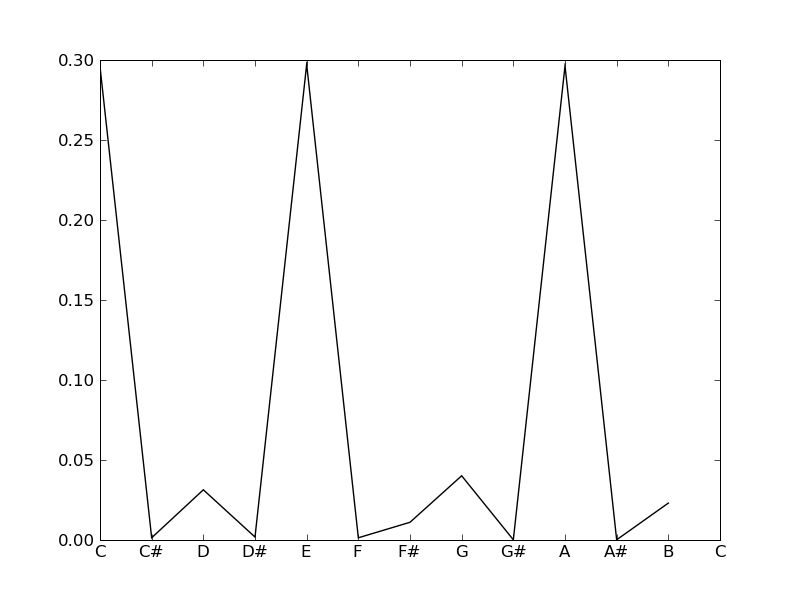
\includegraphics[width=7.5cm]{images/posteriors/posterior-profile-0_5.png} &
        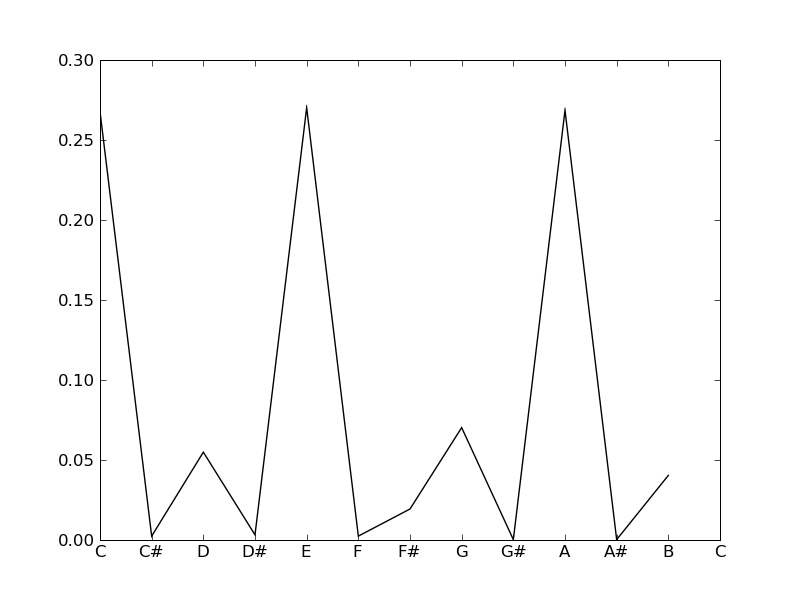
\includegraphics[width=7.5cm]{images/posteriors/posterior-profile-1.png} \\
        $\alpha=0.5$ & $\alpha=1$ \\
    %%	\vspace{1cm} & \\
        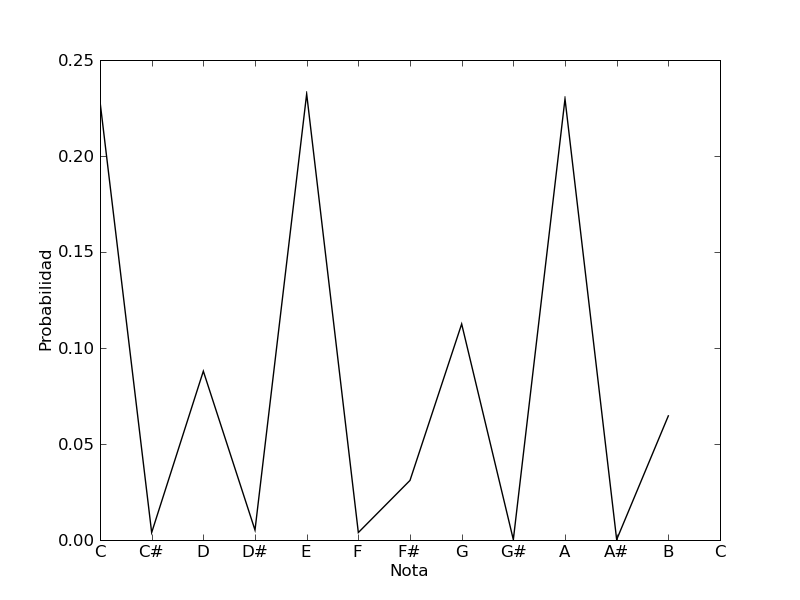
\includegraphics[width=7.5cm]{images/posteriors/posterior-profile-2.png} &
        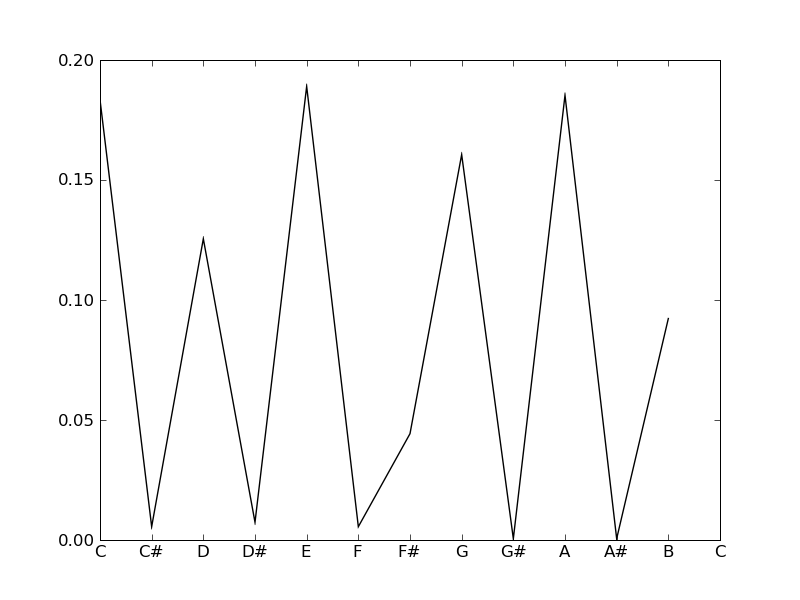
\includegraphics[width=7.5cm]{images/posteriors/posterior-profile-4.png} \\
        $\alpha=2$ & $\alpha=4$ \\
    %%	\vspace{1cm} & \\
        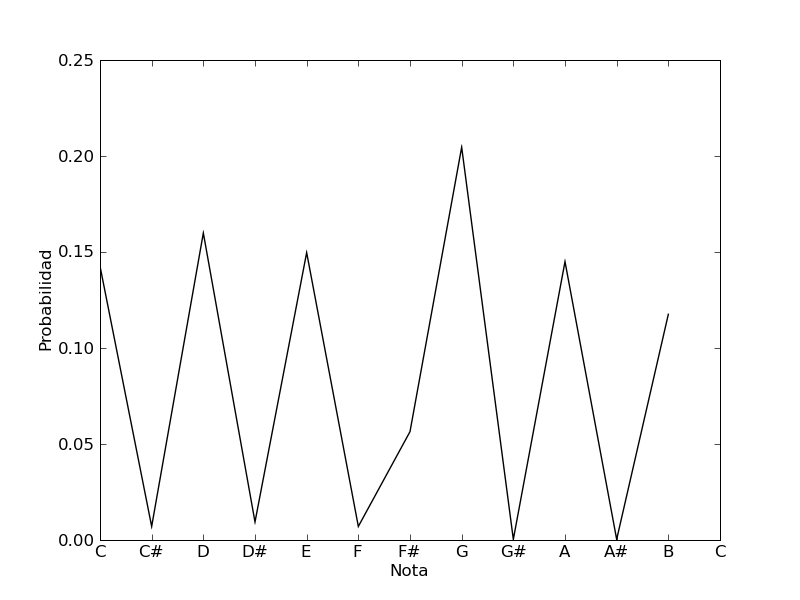
\includegraphics[width=7.5cm]{images/posteriors/posterior-profile-8.png} &
        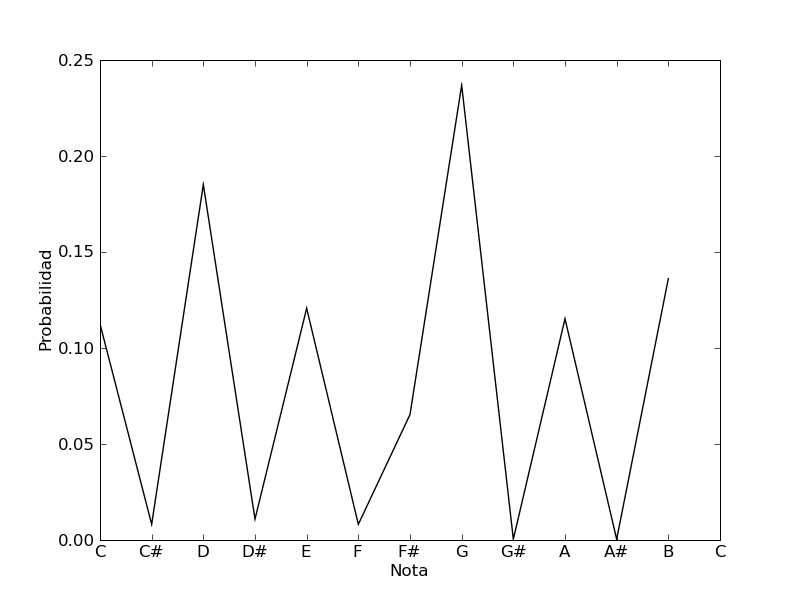
\includegraphics[width=7.5cm]{images/posteriors/posterior-profile-16.png} \\
        $\alpha=8$ & $\alpha=16$ \\
    %%	\vspace{1cm} & \\

        \end{tabular}
        \caption{Distribuciones a posteriori de un contexto arm\'onico para distintos valores de $\alpha$. Se puede ver cuando $\alpha=0.5$ el acorde de La menor 
        domina en el pitch profile, mientras que cuando $\alpha=16$ la distribuci'on predominante responde mayormente a la distribuci'on original con una leve modificaci'on
        en las notas que corresponden al acorde de La menor.}
        \label{fig:pitch_posteriors}
    \end{center}      
\end{figure}

El modelo planteado en esta secci'on hace ciertas asunciones impl'icitas de las que se desea dar detalle. 
Si bien Krumhansl propone al pitch profile Krumhansl como mecanismo para caracterizar la tonalidad en la que se encuentra una pieza, 
podr'ia no ser ser suficiente para generar una melod'ia que sea entendida de la misma forma. 
Como primer variac'ion, en lugar de que la probabilidad de una nota sea la proporci'on de tiempo que esta son'o en el tiempo, 
se podr'ia construir una familia de distribuci'ones indexadas por su duraci'on. 'Esta ser'ia otra forma de reflejar el hecho de que notas que 
suenan m'as tiempo tienden a ser estables.

Obs'ervese que el peso que se le da a cada nota del acorde es igual. En ese caso podr'ia plantearse el modelo en otros t'erminos para permitir un factor de peso, o
alg'un tipo de condici'on que distinga entre cada nota. 

Otra caracter'istica que no es tenida en cuenta en este modelo es el acento m'etrico que recibe una cierta nota. Es sabido que en posiciones m'etricamente m'as fuertes
existen restricci'ones sobre la estabilidad de las notas que se pueden tocar all'i. Nuevamente, una soluci'on podr'ia ser tener una familia de distribuci'ones indexadas
por el acentro m'etrico. Esto mismo ocurre tambi'en con las notas que reciben un acento estructural, sin embargo en la secci'on \ref{sec:phrases} se dar'a una posible
soluci'on a este problema. 

\section{Sobre la detecci\'on de acordes}
Para implementar el modelo propuesto en esta secci'on fue necesario desarrollar una heur'istica para la detecci'on de acordes puesto que la entrada no los trae anotados. 
Esta heur'istica es relativamente simple y se basa en las notas
que suenan en simult'aneo, eliminando las notas que son equivalentes bajo la equivalencia entre octavas. Luego refina el resultado descartando candidatos a acordes que suenan en simult'aneo y no se organizan en saltos de 3 o 4 semitonos, por ejemplo Do, Re, Mi. 

Hay un caso a tener en cuenta, y es que en general, cuando se tocan acordes
con s'eptima, como Do, Mi, Sol, Si$\flat$ se suele obviar la quinta, en este caso Sol. De esta forma, en la partitura se observar'an que las notas Do, Mi, Si$\flat$ suenan
en simult'aneo, y ser'ian falsamente descartadas.  Es por esto que la heur'istica de detecci'on de acordes trata de completar 
con una nota en caso de haber fallado al organizar las notas de a saltos de 3 o 4 semitonos para asi poder inferir el acorde de tr'iada correspondiente (en 
el caso de Do, Mi, Si$\flat$ completar a Do, Mi, Sol, Si$\flat$ e inferir Do, Mi, Sol). 

Queda como trabajo a futuro trabajar con arpegios, es decir, sucesiones de notas que conforman un acorde pero que no son tocadas en simultaneo. 
Se cree que podr'ia atacarse este problema mediante un algoritmo de \emph{changepoint detection}\footnote{El lector interesado en \emph{changepoint detection} refi'erase 
a \cite{adams-mackay-2007}}, para detectar los cambios en el foco tonal. Los algoritmos de changepoint 
detection permiten detectar los puntos de cambio de una sucesi'on de medici'ones en donde la distribuci'on de probabilidades subyacente cambia abruptamente.
A nivel ilustrativo, un ejemplo concreto es el efecto que tiene a la percepci'on de un robot prender la luz de una habitaci'on: Todos las entradas visuales 
sufren un cambio abrupto en su distribuci'on subyacente, de esta forma la estimaci'on que se ten'ia hasta el momento no sirve. En el caso de un cambio
en el foco tonal, la distribuci'on que sufrir'ia un cambio ser'ia la propuesta en esta secci'on, de esta forma, cambios en la distribuci'on a posteriori, indicar'ian
cambios en el foco tonal.

\section{Ejemplos}
Al igual que con el modelo de la m'etrica, se generaron ejemplos de melod'ias siguiendo los modelos definidos en esta secci'on. Para 
cada pieza de entrada se compuso una melod'ia siguiendo un 'unico pitch profile, correspondiente a la tonalidad inferida, y otra
afectando el pitch profile con los acordes detectados. Los ejemplos se encuentran disponibles en 
\url{http://elsonidoq.tzulberti.webfactional.com/examples/?section_name=harmonic_context}.

\section{Modelando l\'ineas mel\'odicas}
\comment{En esta secci'on me focalizo en la partitura como una sucesi'on de alturas}

\subsection{Contextos}
\comment{Aca la idea es explicar que hay que tener en cuenta dos tipos de contextos cuando se trabaja con la melod'ia, uno tiene que ver con cuestiones de las notas que vengo 
tocando, y el otro con el momento en el que estoy de la pieza (que acorde esta sonando). Basicamente, hay un contexto horizontal y otro vertical}

\subsection{La teor\'ia de la Implicaci\'on-Realizaci'on}
\comment{Aca explico mas o menos la teoria de narmour, y cuento como me puede servir para modelar el contexto horizontal}

\subsection{Contexto vertical}
\comment{Yo aca uso un modelo que defini a dedo y que esta todavia sujeto a cambio, me gustaria discutir esto con Favio a ver si esta de acuerdo con lo que estoy haciendo. De todas formas me gustar'ia armar una discuci'on aca. Como contexto vertical, tambien se puede tener en cuenta la tonalidad (en menor medida que el acorde). Me gustaria ver si krumnhansl en su libro cognitive fundations of musical pitch me podria dar algo sobre como llenar esta parte o como hacer un modelo mas interesante (no se si quiero hacer un modelo mas interesante de todas formas =p)}

\subsection{El modelo}

\subsubsection{La cadena de Narmour}
\comment{aca la idea es explicar la cadena de markov de los intervalos de narmour}

\subsubsection{Combinaciones convexas}
\comment{Aca explico como las combinaciones convexas de ciertas distribuciones de probabilidad me determinan el contexto armonico}

\subsection{El proceso generativo}
\comment{Aca tengo que explicar el problema de mezclar estos dos modelos no es trivial, porque se te podria trabar el proceso porque llega a un callejon sin salida, y muestro
como deber'ia ser el proceso compuesto posta}

\section{El modelo compuesto}
Utilizando los modelos definidos en las secciones \ref{sec:metric_model}, \ref{sec:harmonic_contexts} y \ref{sec:melodic_contour}, es posible definir
un proceso generativo para componer lineas mel'odicas de forma relativamente sencilla. 
%Tener en cuenta que dependiendo de la elecci'on del modelo de contorno mel'odico, la cadena de Narmour o la distribuci'on de Narmour, el algoritmo se ver'a
%afectado. El primer modelo permite elegir un conjunto de notas candidatas, mientras que el segundo permite incorporar dentro de una distribuci'on de 
%probabilidades el modelo de contornos melodicos con el modelo del contexto arm'onico. 
A continuaci'on se definir'a el algoritmo exhibiendo el pseudoc'odigo para que quede en una representaci'on compacta: 
para cada nota a generar, el modelo de la r'itmica elejir'a su duraci'on, mientras que el modelo de Narmour en conjunto con el de contexto arm'onico 
elejir'an la altura a tocar en funci'on del 'ultimo intervalo tocado.

\begin{algoritmo}
create_melody(rhythm_model, harmonic_context, contour_model, 
              total_duration, available_notes, context)
    notes := []
    while last_note.end < total_duration
        new_duration := rythm_model.next_duration()

        pitch_distribution= {}
        for note in available_notes
            prob := harmonic_context.get_prob(note)*contour_model.get_prob(note, context)
            pitch_distribution[note] := prob 

        pitch_distribution := normalize(pitch_distribution)
        new_pitch := pick(pitch_distribution)

        last_note := Note(last_note.start, new_duration, new_pitch)
        notes.append(last_note) 

        n1, n2 := context
        context := (n2, last_note)

    return notes
\end{algoritmo}

De esta forma se puede expresar en t'erminos probabil'isticos la elecci'on total de cada nota. Sean $d_j$ la sucesi'on de duraci'ones y $n_j$ 
la sucesi'on de notas, y $\theta$ el vector de par'ametros del contexto arm'onico, entonces la probabilidad de una nota estar'a dada por:

$$P(d_j, n_j | d_{j-1}, n_{j-1}, n_{j-2}) = P(d_j|d_{j-1})P(F_1(n_{j-2}, n_{j-1}, n_j), \cdots, F_k(n_{j-2}, n_{j-1}, n_j)) P(n_j | \theta)$$


\chapter{Modelos jer\'arquicos}
\label{cap:jerar}
\label{cap:modelos_jerarquicos}
\section{Un modeo parcial para frases}
\label{sec:phrases}
Los modelos propuestos hasta el momento est'an focalizados en interacciones nota a nota. Sin embargo, es sabido que la m'usica
tiene una estructura jer'arquica. En esta secci'on se trabajar'a un poco con un elemento de 'indole jer'arquico: la frase. 

Antes de intentar modelar una frase es importante tratar de entender de qu'e se trata este objeto a modelar. El fraseo es una
noci'on complicada de definir, y es por esto que no existe una 'unica definici'on. William Rothstein en su libro \texttt{Phrase Rhythm 
in Tonal Music}, describe las dos mejores, seg'un su criterio, definiciones de frases. Comienza citando al compositor contemporaneo
Roger Sessions: 

\begin{quote} 
[\ldots] What, for instance, is a so-called `musical phrase` if not the portion of music that must be performed, so to speak, 
without letting go, or figuratively, in a single breath?. [\ldots] The phrase is a constant movement towards a goal - the cadence.
\end{quote}

Si bien esta definici'on lejos est'a de permitir construir un modelo generativo para frases, hay dos nociones que son interesantes. 
La primer noci'on es la del respiro: Una frase no puede ser arbitrariamente larga, tampoco puede ser arbitrariamente corta. La 
segunda, es que la frase tiene un \emph{goal}(meta), y este \emph{goal} es la cadencia.%\alert{como defino cadencia?}. 

Luego Rothstein contin'ua citando la definici'on de Peter Westergaard quien distingue dos conjuntos de alturas, y define
a la frase como un movimiento entre estos dos conjuntos de forma tal que se cumplan las siguientes tres propiedades:
\begin{enumerate}
 \item Uno espera el segundo conjunto de alturas
 \item Uno tiene alguna noci'on de cuando este segundo conjunto ocurrir'a
 \item Una vez que el segundo conjunto de alturas ocurri'o, uno sabe que la frase lleg'o donde quer'ia ir
\end{enumerate}


Estas dos definiciones comparten la noci'on de meta; en la definici'on de Sessions, la meta es la cadencia y en la Westergaard 
es el segundo conjunto de notas.  En lo que sigue se propone un modelo que para tratar de capturar parcialmente esta nocion de frase.

\subsection{Las notas de apoyo}
Siguiendo las definiciones
de frase mel'odica vistas en la secci'on anterior, parece ser que la noci'on de meta es una noci'on importante, y que esta meta
est'a relacionada con la armon'ia de la pieza en cuesti'on. 

Tomando la definici'on de Westergaard, para poder hablar de frase es necesario primero saber cuales son los dos conjuntos de 
alturas entre los cuales la frase va a desplazarse. La forma m'as sencilla es pensar estos dos conjuntos como dos acordes sucesivos
y que la melod'ia que transcurre en un acorde en realidad est'a apuntanto hacia el acorde siguiente. Por supuesto
esta es una simplificaci'on, puesto que de la misma forma que existe una jerarqu'ia a nivel notas, existe tambi'en una jerarqu'ia
en la progresi'on arm'onica: ciertos acordes cumplen un rol estructurante mientras que otros cumplen un rol decorativo. Tambi'en
existen acordes que si bien no son iguales, en ciertos contextos se los puede utilizar como \emph{substitutos}. 

Esta elecci'on de la frase como camino entre dos acordes sucesivos tampoco tiene en cuenta de forma directa la restricci'on 
que impone sobre la duraci'on de una frase la definici'on de Sessions, sin embargo es de esperarse que la duraci'on de los acordes de una pieza musical
no sea excesivamente larga ni corta. 

De esta forma, se propone como modelo tomar, para cada acorde, una \emph{nota de apoyo}. Esta nota de apoyo ser'a la meta de 
la frase. Es importante que las notas de apoyo \emph{sean parte} de la frase que se est'a componiendo, es decir, las notas
de apoyo no pueden estar desconectadas del modelo probabilistico que vaya a elejir las notas anteriores y posteriores a la misma. 
Esto se puede expresar como propiedades en t'erminos del modelo que asigna probabilidades a las alturas. 
Estas propiedades descartar'an algunas frases y otras no, y se desea, dentro de las frases que restan, elejir una con probabilidad
proporcional a la que esta ten'ia en el conjunto original de frases. 

Esto en principio podr'ia ser exponencial, ya que la cantidad de posibles frases crece exponencialmente con la longitud de la frase.
Sin embargo, se puede aprovechar la localidad de los principios de Narmour para construir un algoritmo m'as eficiente.  

A continuaci'on se muestra c'omo construir este modelo. 


\subsection{Construcci\'on del submodelo}
\label{sec:phrase_model}
A continuaci'on se definir'a formalmente el problema, y luego se dar'a un algoritmo para resolverlo.

Se cuenta con un modelo que asigna probabilidades a notas seg'un la historia de las 'ultimas dos notas, $P(n_3 | n_1, n_2)$. Si bien se puede generalizar a $k$ notas,
la construcci'on quedar'ia menos clara, y el hecho es que se utilizar'a con solo 2 notas. Sup'ongase adem'as que se encuentra en un contexto formado por las notas 
$n_1, n_2$, y se desea generar una frase mel'odica de $d$ notas, de forma tal que se cumpla una cierta propiedad $M$ (middle) sobre la probabilidad de tocar las notas
del medio de la frase, y cierta propiedad $S$ (support) sobre la nota de apoyo de la siguiente frase. Por ejemplo, $S$ podr'ia restringir a 
que la nota de apoyo tenga una probabilidad alta en su contexto: $S(n_1, n_2, n_f): P(n_f | n_1, n_2) = \max_{(n'_1, n'_2)}{P(n_f | n'_1, n'_2)}$.

Como no todas las melod'ias de $d$ notas van a garantizar esto, se desea descartar todas las melod'ias que no lo garantizan y construir un nuevo modelo, en donde
solo se puedan construir las melod'ias que cumplan con los predicados en cuesti'on. Por 'ultimo, se desea tambi'en que la probabilidad de estas l'ineas mel'odicas 
que satisfacen los predicados, sea proporcional a la asignada por el modelo original. 

La forma en la que se atacar'a este problema, es mediante una sucesi'on de conjuntos indexados por el contexto, la nota final y cuantas notas le queda
a la frase. Estos conjuntos tendr'an la propiedad de que cualquier nota elejida de ellos garantizar'a la existencia de una continuaci'on de la longitud correspondiente 
 y que \emph{lleve a buen puerto}. Utilizando esta propiedad, es posible implementar un algoritmo eficiente para elejir la frase dentro del submodelo. 

Para poder utilizarlo sin cuidado habr'a que demostrar la correctitud de este argumento, demostrando que cualquier frase mel'odica del submodelo se puede construir
utilizando esta serie de conjuntos. Por 'ultimo, la asignaci'on de probabilidades utilizar'a el modelo original, renormalizando en la sucesi'on de conjuntos. De esta 
forma la probabilidad ser'a proporcional al modelo original.

Tomando $M$ y $S$ como restricciones sobre las l'ineas mel'odicas, s'olo ser'an v'alidas las l'ineas $n_1, \cdots, n_k, n_f$ que cumplan con

$$  S(n_{k-1}, n_k, n_f) \land \forall i, i\leq k-2 \Rightarrow M(n_i, n_{i+1}, n_{i+2})$$

Se puede dar una definici'on equivalente definiendo la funci'on $Poss$, que determina las notas suceptibles a ser notas de apoyo dado una cierta historia determinada por al menos dos notas.

\begin{definition}
\label{def:poss}
Sean $n_1, \cdots, n_k$ una sucesi'on de notas, $k\geq2$, se define
\begin{align*}
Poss(n_1, n_2, \cdots, n_k)= \left\{
 \begin{array}{rl}
  \phi & \text{si } \neg valid(n_1, \cdots, n_k) \\ %\exists i < k-1 \text{ tal que } \neg M(n_i, n_{i+1}, n_{i+2}) \\
   \{n_f / S(n_{k-1}, n_k, n_f)\} & \text{si no}
 \end{array} \right.
\end{align*}

Donde $valid(n_1, \cdots, n_k) = \forall i, i\leq k-2 \Rightarrow M(n_i, n_{i+1}, n_{i+2})$
\end{definition}

Se define inductivamente la funci'on $Must(n_1, n_2, n_f, d)$, que dado un contexto $n_1, n_2$ determina el conjunto de notas que habr'a que tocar, de forma tal
que $d$ notas despu'es, la probabilidad de la nota $n_f$ cumpla con $S$ de la siguiente forma:
\begin{definition}
\label{def:must}
\begin{align*}
Must(n_1, n_2, n_f, 1)=& \{n_3/ S(n_2, n_3, n_f) \land M(n_1, n_2, n_3)\}\\
Must(n_1, n_2, n_f, d)=& \{n_3/ Must(n_2, n_3, n_f, d) \neq \phi \land M(n_1,n_2, n_3)\}
\end{align*}
\end{definition}


\ \newline \textbf{Teorema.}
A continuaci'on se demuestra por inducci'on en $d$ que 
$$n \in Must(n_1, n_2, n_f, d) \Leftrightarrow \exists n'_1, \cdots, n'_{d-1} \text{ tales que } n_f \in Poss(n_1, n_2, n, n'_1, \cdots, n'_{d-1})$$

\ \newline \textbf{Demostraci'on.}

Cuando $d=1$
\begin{align*}
n \in Must(n_1, n_2, n_f, 1)   & \Leftrightarrow n \in \{n_3/ S(n_2, n_3, n_f) \land M(n_1, n_2, n_3)\} \\
                               & \Leftrightarrow S(n_2, n, n_f) \land M(n_1, n_2, n)   \\
                               & \Leftrightarrow n_f \in Poss(n_1, n_2, n)
\end{align*}

Suponiendo ahora que el predicado vale para $d$, 
\begin{align}
n \in Must(n_1, n_2, n_f, d+1)   & \Leftrightarrow n \in \{n_3/ Must(n_2, n_3, n_f, d) \neq \phi \land M(n_1,n_2, n_3)\} \nonumber \\
                                 & \Leftrightarrow Must(n_2, n, n_f, d) \neq \phi \land M(n_1,n_2, n) \nonumber \\
                                 & \Leftrightarrow \exists n'_1 \text{ tal que } n'_1 \in Must(n_2, n, n_f, d) \land M(n_1,n_2, n) \label{eq_must}
\end{align}

Utilizando la hip'otesis inductiva sabemos que 
$$  n'_1 \in Must(n_2, n, n_f, d) \Leftrightarrow \exists n'_2, \cdots, n'_{d} \text{ tales que } n_f \in Poss(n_2, n, n'_1, n'_2, \cdots, n'_{d})$$

Por lo tanto la equaci'on \ref{eq_must} es equivalente a
$$ \exists n'_1, n'_2, \cdots, n'_d \text{ tal que } n_f \in Poss(n_2, n, n'_1, \cdots, n'_d) \land M(n_1,n_2, n) $$
Lo 'unico que resta por demostrar es que 
$$ n_f \in Poss(n_2, n, n'_1, n'_2, \cdots, n'_d) \land M(n_1,n_2, n) \Leftrightarrow n_f \in Poss(n_1, n_2, n, n'_1, n'_2, \cdots, n'_d)$$
lo cual es v'alido por la definici'on de $Poss$, demostrando lo que se quer'ia demostrar$\qed$


Con esta definici'on, se define el proceso generativo de la siguiente forma:

\begin{algoritmo}
play_phrase(n1, n2, nf, d, prob_model)
    answer := []
    context := (n1, n2)
    para i desde d hasta 1 hacer
        n1, n2 := context
        candidates := Must(context, nf, i)
        n3 := pick(candidates, prob_model)
        answer.append(n3)
        context := (n2, n3) 
\end{algoritmo}

Es importante notar que para que este algoritmo funcione, se necesita de alguna forma elejir las primeras dos notas. La elecci'on se realiza a trav'es de 
marginalizar los contextos de la siguiente forma:

$$P(n_1, n_2) \propto \sum_{n_3}P(n_1,n_2|n_3)P(n_3)$$



\subsection{Sobre los predicados $S$ y $M$}
\label{sec:must_predicates}
La definici'on de los predicados $S$ y $M$ son de crucial importancia, puesto que de definirlos de forma incorrecta resultar'a en un modelo vacio, 
es decir dados $n_1$ y $n_2$, ocurrir'a que no exista continuaci'on que permita tocar una nota de apoyo al final. 
Es por eso que se desean predicados que permitan definir restricciones, pero al mismo tiempo garantizen que siempre se puede tocar algo.

Una primera aproximaci'on que se tom'o fue definir 
$$S(n_1, n_2, n_3) = P(n_3 | n_1, n_2) \geq X\%$$

El problema ahora es determinar
el valor $X$. Como las probabilidades definidas por el modelo de Narmour estan formadas por un producto de cada uno de los principios, habria 
que considerar esto para la elecci'on de $X$. Adem'as, la elecci'on de un umbral no deja margen para la expermientaci'on con frases
m'as o menos probables puesto que no es facil de controlar el hecho de que el modelo no se haga vacio. 
Por estas razones se descarto la idea de comparar la probabilidad dada por el contexto con una constante. 

Una propiedad deseable de un esquema para predicados $S$ y $M$ es que existan dos casos particulares, 
donde uno corresponda a la melod'ia m'as probable
y otro corresponda a eliminar la restricci'on de estos predicados, y adem'as garantize siempre la existencia de una frase. 

Un esquema que encaja dentro de este marco es un predicado que compare la probabilidad $P(n_3 | n_1, n_2)$ con un 
$V_p$ percentil, es decir, el valor que deja s'olo al $p\%$ de las notas m'as probables.  De esta forma, si el contexto tiene muchos valores probables, 
el percentil se ajustar'a m'as alto, y lo mismo para contextos menos probables.

Hay que tener en cuenta que dado que las observaciones son todas discretas, ser'a frecuente el caso donde 
se asigne exactamente la misma probabilidad a m'as de un evento. En ese caso no se podr'a garantizar un $p\%$ puesto que ser'ia arbitrario
elejir un evento por sobre otro si tienen la misma probabilidad, sin embargo, no se considera que esto sea un mayor problema. Adem'as, este predicado nunca dejar'a un conjunto vac'io, y si se lo define con cuidado, se puede obtener
el comportamiento de la melod'ia m'as probable, cambiando el predicado en el caso de $0\%$.

\subsection{Ejemplo}
En la Figura \ref{fig:unfinished_phrase} se exhiben los compases 6, 7 y 8 de una melod'ia generada a partir de la Danza Alemana WoO 13 N 11 
de Beethoven utilizando el percentil 0. Sup'ongase que se ha generado la melod'ia hasta donde se muestran los signos de interrogaci'on. 
La nota que se encuentra luego de los signos de interrogaci'on es la nota tomada como punto de apoyo para la frase siguiente.

\begin{imagen}
    \file{images/figura_nueva_pregunta.png}
    \labelname{fig:unfinished_phrase}
    \desc{ Un fragmento de una melod'ia donde ya se eliji'o la pr'oxima nota (Mi) de apoyo y restan tocar dos notas.}
    \width{5cm}
\end{imagen}

La meta de que la nota Mi sea fuertemente implicada hace que se establezcan restricciones sobre las dos notas que faltan tocar. 
Siendo que estas notas se encuentran restringidas por el predicado $S$, en la figura \ref{fig:narmour_arrival} se presenta cual ser'ia 
la probabilidad de la nota de apoyo (Mi) para las distintas posibilidades de las notas que est'an marcadas con signo de interrogaci'on. 
Como el percentil utilizado en este caso es el percentil 0, s'olo las notas de la zona marcada con rojo en la figura \ref{fig:narmour_arrival}
pueden ser utilizadas antes que la nota de apoyo. Asimismo, estas notas, al proceder de un cierto contexto mel'odico 
(representado por las dos notas anteriores, La y Mi), deber'an ser elejidas tambi'en a partir de la distribuci'on de probabilidad 
que el modelo compuesto instancie en tal contexto (las notas La y Mi). 

\begin{imagen}
    \file{images/arrival_narmour_64.png}
    \labelname{fig:narmour_arrival}
    \desc{Probabilidad de la nota de apoyo (Mi) para las dos notas anteriores. En el eje X se muestra la primer nota, 
    y en el eje Y se muestra la segunda}
    \width{13cm}
\end{imagen}

\begin{imagen}
    \file{images/narmour_restricted_69_64.png}
    \labelname{fig:narmour_restricted}
    \desc{Probabilidad de la nota de apoyo (Mi) para las dos notas anteriores. En el eje X se muestra la primer nota, y en el eje Y se muestra la segunda }
    \width{13cm}
\end{imagen}

La distribuci'on de probabilidad presentada en la figura \ref{fig:narmour_restricted}, no corresponde al modelo compuesto solamente, sino 
que por sobre este se le aplican las restricciones exhibidas en la figura \ref{fig:narmour_arrival}, de esta forma s'olo las notas que 
pertenecen a la zona marcada con rojo en la figura \ref{fig:narmour_arrival} tienen probabilidad distinta de cero en la figura \ref{fig:narmour_restricted}.

N'otese que si bien se podr'ia considerar que los valores num'ericos de las probabilidades son bajos, hay que tener en cuenta que lo 
importante es la proporci'on que hay entre estos valores. Es decir, en el gr'afico se puede ver que las dos continuaciones m'as 
probables son o bien tocar las notas Do$\sharp$ y luego Re o bien tocar las notas La$\sharp$ y luego F$\sharp$. Estas dos continuaciones 
tienen cada una una probabilidad aproximadamente de $1.37\times10^{-5}$ y $4.51\times10^{-6}$, que si bien en t'erminos absolutos es 
un valor pequeño, la continuaci'on m'as probable es aproximadamente $3.04$ m'as probable que la que le sigue. 

\subsection{Trabajo a futuro: silencios}
Los modelos propuestos hasta el momento no toman en cuenta al silencio. 
%\cite{PaieThesis} incorpora el silencio como un elemento m'as
%dentro de la generaci'on de alturas, sin embargo se considera que el silencio no es un elemento con el mismo status que las alturas. 
El silencio cambia su comportamiento seg'un el contexto donde este aparezca, y si bien esto tambi'en pasa con las notas, las reglas que se
aplican a este 'ultimo son otras. 

\cite{Margulis08} distingue dos roles del silencio dependiendo del contexto. Si la sonoridad gobernante est'a dada por un acorde de dominante
o de subdominante, un silenci'o aumenta la tensi'on que ya de por s'i generan dichos acordes, mientras que si la sonoridad gobernante
esta dada por un acorde de t'onica, el silencio disminuir'a m'as la tensi'on. Es por esto que se considera que los silencios no tienen 
un status igual que el resto de las notas, y su status es de tinte jer'arquico.

Se propone trabajar en el futuro incorporando los silencios como una componente de 'indole jerarquica conjuntamente con el fraseo.

\section{Generando motivos}
Hasta el momento se exhibieron modelos capaces de cuantificar la estabilidad de una nota en un cierto contexto, de generar una r'itmica que
respete el acento m'etrico del tema original. Utilizando estos modelos y a partir de algunas definiciones de una frase musical, se mostr'o c'omo es posible
generar frases mel'odicas que tengan un objetivo. Estos modelos contribuyen a la generaci'on de una l'inea mel'odica coherente. Con estos modelos es posible
generar una idea musical, sin embargo, gran parte de la coherencia musical radica en la repetici'on de ideas. Es por esto que se requiere trabajar con \emph{motivos}. 

Un motivo es una idea de alguna forma recurrente, que se destaca en un fragmento musical. Esta idea puede estar dada por una repetici'on parcial de una c'elula 
r'itmica o un contorno mel'odico, aunque no se limita solamente a ello. Cuando una idea de estas caracter'isticas ocurre, sela refiere en t'erminos
de elaboraci'ones mot'ivicas, y lo que las caracteriza es que al escuchar una elaboraci'on mot'ivica se evoca la idea original.

\cite{Deliege87} propone una teor'ia a la que denomina ``teor'ia de la extracci'on de pistas''\footnote{Cue Extraction Theory} en donde postula la existencia de un mecanismo cognitivo de 
extracci'on de pistas 
que es creado a partir de la escucha atenta. Estas pistas son utilizadas como etiquetas para la retenci'on de grupos (utilizando la definici'on de 
\cite{LerdahlJackendoff83}). \cite{Deliege90} relaciona el grado el
de redundancia de una pieza con el nivel de atenci'on que 'esta le demanda al oyente. A nivel extremo, cuando una pieza musical contiene demasiadas estructuras 
repetitivas s'olo un m'inimo de atenci'on es requerido, derivando progresivamente a una escucha completamente pasiva. Sin embargo cuando hay demasiadas 
pistas debido a una r'apida acumulacion de informaci'on o a la escasez de estructuras peri'odicas, el nivel de atenci'on demandado es tan grande que 
termina por hacer desistir al oyente de prestar atenci'on a la pieza musical.

Las composiciones generadas por los modelos propuestos hasta el momento recaen mayormente en el segundo grupo, puesto que la probabilidad de que se escuche
una repetici'on es pr'acticamente nula. De esta forma, el objetivo de esta secci'on es exhibir c'omo se puede aumentar la probabilidad de una repetici'on.



\subsection{Repetici\'on exacta de partes}
\label{sec:crp_model}
Una primera aproximaci'on para generar motivos es bajo ciertas circunstancias repetir exactamente algo que ya se toc'o. Es de esperarse que no pueda repetirse
una parte ya tocada en cualquier lugar del tema, puesto que se desea respetar el contexto arm'onico y las notas de apoyo elegidas. De esta forma, debe
de tomarse como definci'on de contexto para una frase, una que por lo menos respete tanto el acorde como la duraci'on del mismo, puesto que de repetirse una frase, esta 
debe cubrir exactamente el tiempo que abarca el acorde. Otra posibilidad es utilizar el acorde predecesor con el objeto
de modelar la funci'on arm'onica que este estar'ia cumpliendo en el acorde actual. Inclusive se podr'ia agregar el acorde siguiente. Sin embargo, es peligroso modelizar
la funci'on arm'onica de esta forma sin un mecanismo previo de abstracci'on para los acordes, puesto que existen mucho acordes ligeramente distintos entre si que en t'erminos
musicales funcionan como el mismo acorde.

Asumiendo una noci'on de contexto razonable, se podr'ia pensar a una pieza musical como una sucesi'on de contextos. Siendo asi, lo que determinar'ia el proceso generativo para 
la repetici'on exacta de partes es, ante la repetici'on de un contexto, si se repetir'a lo que ya se toc'o en ese contexto, o se har'a
algo nuevo. 

Una posible forma de modelar este proceso generativo es utilizando un Restaurant Chino para cada contexto. Dado un cierto Restaurant, en cada mesa se encuentra
escrita una posible frase para el contexto que le corresponde, y el hecho de que se observe en una pieza musical repetidas veces un contexto equivaldr'ia a que lleguen nuevas
personas al Restaurant. Cada persona elegir'a una mesa, y se utilizar'a la partitura que se encuentra en ella para tocar en ese contexto. Si la mesa es una mesa 
nueva esto equivaldr'a a que se componga una nueva frase para este contexto, aunque se puede pensar como si la partitura siempre hubiera estado en la mesa, s'olo 
no fue observada hasta el momento.  

Por ejemplo, sup'ongase que se cuenta con una pieza cuya sucesi'on de contextos es \texttt{A B B A A B C}. Dado que el conjunto de posibles contextos es
\texttt{A, B} o \texttt{C}, habr'a tres Restaurantes en el sistema. El hecho de que el tema comienze con la parte \texttt{A} indica que llega una persona al 
Restaurant asociado a esta parte. De esta forma, en la figura \ref{fig:crp_example} se exhibe una posible disposici'on de clientes en los tres Restaurantes 
una vez que el tema ha finalizado:

\begin{imagen}
    \file{images/crp_example.png}
    \labelname{fig:crp_example}
    \desc{Posible configuraci'on final de los Restaurantes Chinos correspondientes a los contextos \texttt{A, B} y \texttt{C}}
    \width{10cm}
\end{imagen}


Esto indica que para la parte \texttt{A} se han tocado 3 frases distintas, y para la parte \texttt{B} se han tocado dos frases distintas. 
N'otese que para la parte \texttt{C} la 'unica alternativa es la que se exhibe en la figura.

Formalmente, dada una sucesi'on de contextos $c_1, \cdots, c_n$, donde se espera que haya $k<n$ contextos distintos, se cuenta con $k$ Restaurantes Chinos indexados por contexto,
es decir, $R_{c_i}$ es el Restaurant correspondiente al contexto $c_i$. 

Recordar la propiedad de clustering establecida en la ecuaci'on \ref{eq:crp_clustering}. Esta propiedad 
establece que, dado el par'ametro de concentraci'on $\alpha$, la esperanza de la cantidad de mesas ocupadas luego del arrivo de $N$ clientes es proporcional a $\alpha\times log(N)$.
De esta forma, el par'ametro $\alpha$ de alguna forma regular'ia el grado de variaci'on al que se refiere \cite{Deliege90}. 

A modo de ejemplo, sup'ongase un valor de $\alpha=100$ y una sola persona
en el restaurant. La probabilidad de que alguien se siente en una mesa nueva ser'ia 100 veces mayor a que repita la mesa donde est'a el primer cliente. Sin embargo, si $\alpha=0.5$, 
la probabilidad de que el segundo cliente elija la mesa donde est'a el primero, es el doble a que elija una nueva mesa.

Existe una salvedad t'ecnica que es importante aclarar. Hay que entender a este como un mecanismo que aumenta considerablemente la probabilidad de que se repita una parte ya tocada,
sin embargo, el hecho de que se elijan dos mesas distintas no implica que se vayan a tocar dos partes distintas, puesto que la generaci'on de la parte correspondiente
a cada mesa es independiente. Adem'as, el hecho de que la duraci'on del contexto sea finita, que el modelo para la r'itmica sea b'asicamente una expresi'on regular y 
las notas posibles para tocar por el instrumento sean tambi'en finitas (en general no mucho m'as que dos octavas) hace que las posibles frases para un cierto contexto
sean finitas. Dicho esto, si se repitiera demasiadas veces una parte, eventualmente la cantidad de mesas elegidas superar'ia a la cantidad de partes disponibles
para tocar en ese contexto y se empezar'ian a repetir partes por una cuesti'on de finitud. 

Este problema hay que tenerlo presente en la elecci'on de los predicados $S$ y $M$ de la secci'on \ref{sec:must_predicates}, puesto que en t'erminos pr'acticos esto 'unicamente
ocurrir'ia si estos predicados son demasiado restrictivos, en cuyo caso el efecto de los Restaurantes Chinos ser'ia por dem'as marginal.


\subsection{Repetici\'on aproximada de partes}
Otra aproximaci'on posible (y m'as adecuada a lo que efectivamente pasa en la realidad) es, en lugar de repetir exactamente una frase, repetir una frase que de alguna forma se parezca. 
A saber por el autor, no existe una definici'on operativa sobre qu'e es un motivo musical. Sin embargo se sabe que las elaboraciones mot'ivicas se relacionan 
con patrones sobre las caracter'isticas ya modeladas en las secci'ones anteriores. Siendo as'i, una alternativa es, dada una frase $F$ tocada anteriormente y un modelo $M$ que la gener'o, 
construir un nuevo modelo $M'$ que genere elaboraci'ones motivicas de esta. Se proponen dos propiedades que el modelo de elaboraciones mot'ivicas deber'ia cumplir:

\begin{itemize}
 \item Repetici'on: La probabilidad de la frase $F$ seg'un $M'$ debe ser ``considerablemente'' alta. 
 \item Elaboraci'on: Si en el proceso de generar una frase $F'$ seg'un $M'$ eventualmente se toca algo que no pertenece a $F$, entonces la probabilidad de que la frase $F'$ se reacople a $F$ es alta.
\end{itemize}

La propiedad de \emph{repetici'on} se podr'ia modelar dentro de un marco bayesiano tomando el modelo original como un prior y la frase que actualize a un posterior. 
Eligiendo adecuadamente el factor de peso que tiene el prior sobre la observaci'on de la frase, el comportamiento de que lo m'as probable sea repetir la frase se cumple, 
sin embargo, la propiedad de \emph{elaboraci'on} no estar'ia modelada.

T'omese por ejemplo el modelo de markov de la r'itmica de la figura \ref{fig:rythm_mzt2}. Sup'ongase que se realiz'o la siguiente caminata sobre el modelo:

$$0, 2, 2+\frac{1}{2}, 0$$

Mediante un posterior aplicado correctamente, podr'ia sesgarse a que si se est'a comenzando la frase, entonces la probabilidad de ir a $2$ es mucho m'as alta que la probabilidad de resto
de las transiciones, sin embargo est'a totalmente subespecificado que es lo que ocurrir'ia en el caso que se elijiera ir a $1$ o a $\frac{1}{4}$. 

Es por esto que se propone como trabajo a futuro investigar en una metodolog'ia para la construcci'on de modelos para elaboraci'ones mot'ivicas.


%\section{El modelo completo}
%En esta secci'on se har'a un breve resumen sobre como todos los modelos planteados hasta el momento interactuan entre s'i para generar finalmente una melod'ia.
%En la figura \ref{fig:arquitectura} se exhibe un diagrama. En este, hay dos tipos de nodos. Los nodos circulares representan datos que se leen o que se escriben, y los nodos
%circulares representan modelos. A continuaci'on se enumeran las responsabilidades de cada modelo:
%
%
%\begin{imagen}
%    \file{images/arq.png}
%    \labelname{fig:arquitectura}
%    \desc{Descripci'on gr'afica de la arquitectura utilizada}
%    \width{10.5cm}
%    \position{!h}
%\end{imagen}
%
%\begin{itemize}
% \item Pitch Profile: Construye el pitch profile definido en la secci'on \ref{sec:pitch_profile}.
% \item Chord Detection: Aplica la heur'istica de detecci'on de acordes.
% \item Contour Patterns: Calcula el modelo definido en la secci'on \ref{sec:contour_model}.
% \item Notes Distribution: A partir del Pitch Profile y del acorde actual construye la distribuci'on de notas que aplica al contexto actual seg'un se defini'o en la secci'on \ref{sec:harmonic_context_model}.
% \item Phrase Repetition: Utilizando el Restaurant Chino correspondiente al acorde actual, se elije un identificador para la parte actual como 
% se defini'o en la secci'on \ref{sec:crp_model}.
% \item Phrase Rhythm: Utilizando la duraci'on determinada por el acorde actual y el identificador determinado por la etapa de Phrase Repetition se 
% genera una frase r'itmica como se defini'o en la secci'on \ref{sec:rythm_model}.
% \item Pitch Phrase: Utilizando la r'itmica generada por la etapa de Phrase Rhythm, se llenan los \emph{slots} que esta determina, utilizando
% como contexto arm'onico el determinado por Notes Distribution y utilizando como restricci'ones para el contorno mel'odico las determinadas por
% Contour Patterns utilizando el algoritmo definido en la secci'on \ref{sec:phrase_model}.
%\end{itemize}
%

\chapter{Experimentos}
\label{cap:experiments}
\section{Experimentos}
\subsection{C\'omo construir experimentos que sirvan}
\comment{aca la idea es armar una discuci'on tratando de llegar a deducir los experimentos que tengo que hacer del objetivo de la tesis}

\section{Resultados}

\section{Trabajo futuro}


%\appendix
%\noappendicestocpagenum
%\addappheadtotoc
%
%% Adjustments headers
%\pagestyle{fancy}
%\fancyhead[LO]{\leftmark}
%\fancyhead[RE]{\emph{Ap\'endice \thechapter}}
%\renewcommand{\headrulewidth}{0.5pt}
%
%\section{El problema de programar}
\comment{aca la idea es contar cosas sobre mi experiencia programando algo tan grande}


%\bibliographystyle{apalike}
\bibliography{tesis}
\end{document}

